\documentclass{eieproyecto}
\usepackage{gensymb}
\usepackage{epstopdf}
\usepackage{verbatim}
\usepackage{listings}
\usepackage{color}
\usepackage{subcaption}
\definecolor{dkgreen}{rgb}{0,0.6,0}
\definecolor{gray}{rgb}{0.5,0.5,0.5}
\definecolor{mauve}{rgb}{0.58,0,0.82}

\definecolor{lightgray}{rgb}{0.95, 0.95, 0.95}
\definecolor{darkgray}{rgb}{0.4, 0.4, 0.4}
\definecolor{purple}{rgb}{0.65, 0.12, 0.82}
\definecolor{editorGray}{rgb}{0.95, 0.95, 0.95}
\definecolor{editorOcher}{rgb}{1, 0.5, 0} % #FF7F00 -> rgb(239, 169, 0)
\definecolor{editorGreen}{rgb}{0, 0.5, 0} % #007C00 -> rgb(0, 124, 0)
\usepackage{upquote}
% CSS

%\usepackage{bera}% optional: just to have a nice mono-spaced font
\usepackage{xcolor}
\usepackage{blindtext}
\captionsetup[lstlisting]{position=bottom}
\colorlet{punct}{red!60!black}
\definecolor{background}{HTML}{EEEEEE}
\definecolor{delim}{RGB}{20,105,176}
\colorlet{numb}{magenta!60!black}

\lstdefinelanguage{json}{
	basicstyle=\normalfont\ttfamily,
	numbers=left,
	numberstyle=\scriptsize,
	stepnumber=1,
	numbersep=8pt,
	showstringspaces=false,
	breaklines=true,
	frame=lines,
	backgroundcolor=\color{background},
	literate=
	*{0}{{{\color{numb}0}}}{1}
	{1}{{{\color{numb}1}}}{1}
	{2}{{{\color{numb}2}}}{1}
	{3}{{{\color{numb}3}}}{1}
	{4}{{{\color{numb}4}}}{1}
	{5}{{{\color{numb}5}}}{1}
	{6}{{{\color{numb}6}}}{1}
	{7}{{{\color{numb}7}}}{1}
	{8}{{{\color{numb}8}}}{1}
	{9}{{{\color{numb}9}}}{1}
	{:}{{{\color{punct}{:}}}}{1}
	{,}{{{\color{punct}{,}}}}{1}
	{\{}{{{\color{delim}{\{}}}}{1}
	{\}}{{{\color{delim}{\}}}}}{1}
	{[}{{{\color{delim}{[}}}}{1}
	{]}{{{\color{delim}{]}}}}{1},
}


\lstdefinelanguage{CSS}{
	keywords={color,background-image:,margin,padding,font,weight,display,position,top,left,right,bottom,list,style,border,size,white,space,min,width, transition:, transform:, transition-property, transition-duration, transition-timing-function},	
	sensitive=true,
	morecomment=[l]{//},
	morecomment=[s]{/*}{*/},
	morestring=[b]',
	morestring=[b]",
	alsoletter={:},
	alsodigit={-}
}

% JavaScript
\lstdefinelanguage{JavaScript}{
	morekeywords={typeof, new, true, false, catch, function, return, null, catch, switch, var, if, in, while, do, else, case, break},
	morecomment=[s]{/*}{*/},
	morecomment=[l]//,
	morestring=[b]",
	morestring=[b]'
}

\lstdefinelanguage{HTML5}{
	language=html,
	sensitive=true,	
	alsoletter={<>=-},	
	morecomment=[s]{<!-}{-->},
	tag=[s],
	otherkeywords={
		% General
		>,
		% Standard tags
		<!DOCTYPE,
		</html, <html, <head, <title, </title, <style, </style, <link, </head, <meta, />,
		% body
		</body, <body,
		% Divs
		</div, <div, </div>, 
		% Paragraphs
		</p, <p, </p>,
		% scripts
		</script, <script,
		% More tags...
		<canvas, /canvas>, <svg, <rect, <animateTransform, </rect>, </svg>, <video, <source, <iframe, </iframe>, </video>, <image, </image>
	},
	ndkeywords={
		% General
		=,
		% HTML attributes
		charset=, src=, id=, width=, height=, style=, type=, rel=, href=,
		% SVG attributes
		fill=, attributeName=, begin=, dur=, from=, to=, poster=, controls=, x=, y=, repeatCount=, xlink:href=,
		% CSS properties
		margin:, padding:, background-image:, border:, top:, left:, position:, width:, height:,
		% CSS3 properties
		transform:, -moz-transform:, -webkit-transform:,
		animation:, -webkit-animation:,
		transition:,  transition-duration:, transition-property:, transition-timing-function:,
	}
}

\lstset{%
	% General design
	backgroundcolor=\color{editorGray},
	basicstyle={\small\ttfamily},   
	frame=l,
	% line-numbers
	xleftmargin={0.75cm},
	numbers=left,
	stepnumber=1,
	firstnumber=1,
	numberfirstline=true,	
	% Code design
	identifierstyle=\color{black},
	keywordstyle=\color{blue}\bfseries,
	ndkeywordstyle=\color{editorGreen}\bfseries,
	stringstyle=\color{editorOcher}\ttfamily,
	commentstyle=\color{darkgray}\ttfamily,
	% Code
	language=HTML5,
	alsolanguage=JavaScript,
	alsodigit={.:;},	
	tabsize=2,
	showtabs=false,
	showspaces=false,
	showstringspaces=false,
	extendedchars=true,
	breaklines=true,
	% German umlauts
	literate=%
	{Ö}{{\"O}}1
	{Ä}{{\"A}}1
	{Ü}{{\"U}}1
	{ß}{{\ss}}1
	{ü}{{\"u}}1
	{ä}{{\"a}}1
	{ö}{{\"o}}1
}

%Packages
\usepackage{xspace}
\usepackage{color}

%Colours
%ucr
\definecolor{celesteUCR}{RGB}{65,173,231}
\definecolor{amarilloUCR}{RGB}{249,234,100}
\definecolor{verdeUCR}{RGB}{81,186,69}
%
%tum
\definecolor{blueTUM}{RGB}{0,105,178}
%
\definecolor{redPRIS}{RGB}{180,0,0}
\definecolor{yellowPRIS}{RGB}{240,230,170}
\definecolor{grayPRIS}{RGB}{90,100,140}
\definecolor{blackPRIS}{RGB}{0,0,0}
%
\definecolor{prisred}{RGB}{180,0,0}
\definecolor{prisgrey}{RGB}{180,150,150}
\definecolor{darkgrey}{RGB}{50,60,70}
\definecolor{lightgrey}{RGB}{150,150,150}
\definecolor{labgrey}{RGB}{90,100,140}
\definecolor{labyellow}{RGB}{240,230,170}
\definecolor{prisgray}{RGB}{50,60,70}
\definecolor{prisblack}{RGB}{0,0,0}
\definecolor{prisblue}{RGB}{40,65,140}
\definecolor{ace1}{RGB}{0,150,215}
\definecolor{ace2}{RGB}{0,50,70}
\definecolor{ribBlue}{RGB}{0,100,150}

\definecolor{pris}{RGB}{180,0,0}
\definecolor{prisblue}{RGB}{40,65,140}
% \definecolor{prisgray}{RGB}{107,107,107}
\definecolor{labyellow}{RGB}{240,230,170}
\definecolor{lightgrey}{RGB}{150,150,150}

%Teknovae colors
\definecolor{teknovaeBlack}{RGB}{0,0,0}
\definecolor{teknovaeOrange}{RGB}{255,139,51}
\definecolor{teknovaeGreen}{RGB}{3,204,0}
\definecolor{teknovaeBlue}{RGB}{65,26,255}
%
\definecolor{blackTKN}{RGB}{0,0,0}
\definecolor{redTKN}{RGB}{255,139,51}
\definecolor{greenTKN}{RGB}{3,204,0}
\definecolor{blueTKN}{RGB}{65,26,255}

%Fonts
\DeclareFontFamily{T1}{pbk}{}
\DeclareFontFamily{T1}{pbks}{}
\DeclareFontShape{T1}{pbk}{m}{n}{<->s*pbkl}{}
\DeclareFontShape{T1}{pbks}{m}{n}{<->s*[0.7]pbkl}{}

%Names
\newcommand{\prislab}{{\fontfamily{pbk}\selectfont\textcolor{prisred}{PR}\textcolor{prisblack}{IS}}{\fontfamily{pbks}\selectfont\textcolor{prisgray}{-LAB}}\xspace}
\newcommand{\pris}{Pattern Recognition and Intelligent Systems Laboratory\xspace}
\newcommand{\prises}{Laboratorio de Investigación en Reconocimiento de Patrones y Sistemas Inteligentes\xspace}
\newcommand{\prisfull}{\prislab: \pris}
\newcommand{\prisfulles}{\prislab: \prises}

\definecolor{core1}{RGB}{75,95,115}
\definecolor{core2}{RGB}{220,60,60}
\newcommand{\core}{{\fontfamily{bookman}\sc \textcolor{core1}{C}\textcolor{core2}{o}\textcolor{core1}{re}}\xspace}

\definecolor{excess1}{RGB}{33,180,168}
\definecolor{excess2}{RGB}{190,0,60}
\newcommand{\excess}{{\fontfamily{bookman}\sc \textcolor{excess1}{E}\textcolor{excess2}{x}\textcolor{excess1}{cess}}\xspace}

\definecolor{essence1}{RGB}{90,140,50}
\definecolor{essence2}{RGB}{124,222,50}
\newcommand{\essence}{{\fontfamily{bookman}\sc \textcolor{essence1}{E}\textcolor{essence2}{ss}\textcolor{essence1}{ence}}\xspace}

\newcommand{\bend}{{\fontfamily{bookman}\sc \textcolor{excess2}{B}\textcolor{excess1}{e}\textcolor{excess1}{nd}}\xspace}
\newcommand{\hint}{{\fontfamily{bookman}\sc \textcolor{essence1}{H}\textcolor{essence2}{int}}\xspace}

% PRIS-Lab
% \newcommand{\pris}{Pattern Recognition and Intelligent Systems Laboratory\xspace}
% \newcommand{\prislab}{{\fontfamily{bookman}\sc\textcolor{prisred}{PR}\textcolor{black}{IS\textcolor{prisgray}{-lab}}}\xspace}
% \newcommand{\bcrn}{{\fontfamily{bookman}\sc\textcolor{prisred}{PR}\textcolor{black}{IS\textcolor{prisgray}{-lab}}}\xspace}
% \newcommand{\prisfull}{{\fontfamily{bookman}\sc\prislab}: \pris}
% \newcommand{\prislabfull}{\sc Laboratorio de Investigación en\\\textcolor{redPRIS}{Reconocimiento de Patrones}\\y Sistemas Inteligentes}
\newcommand{\aprs}{{\fontfamily{bookman}\sc APRS}\xspace}
\newcommand{\aprsfull}{{\fontfamily{bookman}\sc\aprs}: Advanced Pattern Recognition System\xspace}
\newcommand{\aprsfulles}{{\fontfamily{bookman}\sc\aprs}: Sistema Avanzado de Reconocimiento de Patrones\xspace}
%
\newcommand{\prissem}{{\fontfamily{bookman}\sc\textcolor{prisred}{PR}\textcolor{black}{IS\textcolor{black}{-Seminar}}}\xspace}
\newcommand{\coloquio}{\textit{Coloquio de Investigación}\xspace}
\newcommand{\ace}{{\fontfamily{bookman}\sc\textcolor{ace1}{A}\textcolor{ace2}{ce}}\xspace}

\newcommand{\sura}{{\fontfamily{bookman}\sc\textcolor{prisred}{S}\textcolor{black}{u}\textcolor{prisblue}{r}\textcolor{prisgray}{á}}\xspace}
\newcommand{\boknama}{{\fontfamily{bookman}\sc Boknama}\xspace}
\newcommand{\iriria}{{\fontfamily{bookman}\sc Iriria}\xspace}

%Networks
\newcommand{\rib}{{\fontfamily{bookman}\sc\textcolor{ribBlue}{RIB}}\xspace}
\newcommand{\ribfull}{\rib: Red de Investigación en Biocomputación\xspace}
\newcommand{\bcrn}{{\fontfamily{bookman}\sc\textcolor{ribBlue}{BcRN}}\xspace}
\newcommand{\bcrnfull}{\bcrn: Biocomputing Research Network\xspace}

\newcommand{\rider}{{\fontfamily{bookman}\sc \textcolor{orange!80!black}{Rider}}\xspace}
\newcommand{\riderfull}{\rider: Red de Investigación y Desarrollo en Eficiencia Energética y Tecnologías en Energía Renovable\xspace}

\newcommand{\ricc}{{\fontfamily{bookman}\sc \textcolor{red!80!black}{R}\textcolor{green!80!black}{I}\textcolor{blue!80!black}{C}\textcolor{prisgray}{C}}\xspace}
\newcommand{\riccfull}{\ricc: Red de Investigación en Computación Científica\xspace}
\newcommand{\scrn}{{\fontfamily{bookman}\sc \textcolor{red!80!black}{S}\textcolor{green!80!black}{C}\textcolor{blue!80!black}{R}\textcolor{prisgray}{N}}\xspace}
\newcommand{\scrnfull}{\scrn: Scientific Computing Research Network\xspace}

%Institutions
\newcommand{\arcoslab}{ARCOS-LAB\xspace}
\newcommand{\arcoslabfull}{\arcoslab: Autonomous Robots and Cognitive Systems Laboratory\xspace}

\newcommand{\clcar}{CLCAR\xspace}
\newcommand{\clcarfull}{\clcar: Conferencia Latinoamericana de Computación de Alto Rendimiento\xspace}

\newcommand{\nsf}{{\fontfamily{bookman}\sc NSF}\xspace}
\newcommand{\nsffull}{\nsf: National Science Foundation\xspace}

\newcommand{\conare}{{\fontfamily{bookman}\sc CONARE}\xspace}
\newcommand{\conarefull}{\conare: Consejo Nacional de Rectores\xspace}

\newcommand{\cenat}{{\fontfamily{bookman}\sc CeNAT}\xspace}
\newcommand{\cenatfull}{\cenat: Centro Nacional de Alta Tecnología\xspace}

\newcommand{\cnca}{{\fontfamily{bookman}\sc CNCA}\xspace}
\newcommand{\cncafull}{\cnca: Co-laboratorio Nacional de Computación Avanzada\xspace}
\newcommand{\cadejos}{{\fontfamily{bookman}\sc\textcolor{black}{cadejos}}\xspace}

\newcommand{\ictp}{ICTP: International Centre for Theoretical Physics\xspace}


\newcommand{\ucr}{Universidad de Costa Rica\xspace}
\newcommand{\eie}{Escuela de Ingeniería Eléctrica\xspace}
\newcommand{\fing}{Facultad de Ingeniería\xspace}

\newcommand{\towhom}{To Whom it May Concern\xspace}
\newcommand{\aquien}{A Quien Corresponda\xspace}

\newcommand{\fourVidTags}{\emph{4vid}\textit{Tags}\xspace}



%Conferences
\newcommand{\ines}{17th IEEE International Conference on Intelligent Engineering Systems -- INES\xspace}
\newcommand{\cinti}{14th IEEE International Symposium on Computational Intelligence and Informatics -- CINTI\xspace}
\newcommand{\sami}{IEEE International Symposium on Applied Machine Intelligence and Informatics -- SAMI\xspace}

%People
\newcommand{\juanD}{Juan Marcos Delgado Zumbado, MLE\xspace}
\newcommand{\juanDjob}{Director}
\newcommand{\juanDwho}{Estimado Sr. Delgado}

\newcommand{\lauraR}{Laura Robles Loaiza, Licda.\xspace}
\newcommand{\lauraRjob}{Unidad de adquisiciones, \os}
\newcommand{\lauraRwho}{Estimada Sra. Robles}

\newcommand{\yamilethF}{Yamileth Figueroa Barahona, MBA.\xspace}
\newcommand{\yamilethFjob}{Directora de la Dirección Financiera, Rectoría\xspace}
\newcommand{\olgaC}{Olga Cordero Quirós\xspace}
\newcommand{\olgaCjob}{Gestora de la Dirección Financiera, Rectoría\xspace}
\newcommand{\electrizarte}{ElectrizArte\xspace}

\newcommand{\oaice}{OAICE\xspace}
\newcommand{\oaicefull}{\oaice: Oficina de Asuntos Internacionales y Cooperación Externa\xspace}
\newcommand{\oaicename}{Oficina de Asuntos Internacionales y Cooperación Externa\xspace}

\newcommand{\julietaC}{Dra. Julieta Carranza Velázquez\xspace}
\newcommand{\julietaCjob}{Directora \oaice\xspace}
\newcommand{\julietaCwho}{Estimada Dra. Carranza\xspace}

\newcommand{\walterM}{Dr. Walter Marín Méndez\xspace}
\newcommand{\walterMjob}{Subdirector \oaicename\xspace}
\newcommand{\walterMwho}{Estimado Dr. Marín\xspace}

\newcommand{\fatimaA}{Fátima Acosta López\xspace}
\newcommand{\fatimaAjob}{Jefe de Sección de Movilidad Académica-Administrativa\xspace}
\newcommand{\fatimaAwho}{Estimada Sra. Acosta\xspace}

\newcommand{\haydeeR}{Haydée Ramos\xspace}
\newcommand{\haydeeRjob}{Académicos Visitantes, Becas Cortas\xspace}
\newcommand{\haydeeRwho}{Estimada Sra. Ramos\xspace}


\newcommand{\osg}{OSG\xspace}
\newcommand{\osgname}{Oficina de Servicios Generales\xspace}
\newcommand{\osgfull}{\osg: \osgname}

\newcommand{\oscarM}{M.Sc. Óscar Mario Molina Molina\xspace}
\newcommand{\oscarMjob}{Director\xspace}
\newcommand{\oscarMwho}{Estimado Sr. Molina\xspace}

\newcommand{\jeffreyD}{Ing. Jeffrey Dimarco Fernández\xspace}
\newcommand{\jeffreyDjob}{Jefe de la sección de transportes\xspace}
\newcommand{\jeffreyDwho}{Estimado Sr. Dimarco\xspace}

\newcommand{\audiP}{Audi Paniagua Gómez\xspace}
\newcommand{\audiPjob}{Sección de transportes\xspace}
\newcommand{\audiPwho}{Estimado Sr. Paniagua\xspace}




\newcommand{\anaAA}{Ana Alfaro Alvarado\xspace}
\newcommand{\anaAAjob}{Gestora de  Becas CU / Consejo de Rectoría / FDI / Membresías\xspace}
\newcommand{\anaAAwho}{Estimada Sra. Alfaro\xspace}

\newcommand{\MIT}{Massachusetts Institute of Technology\xspace}

\newcommand{\tec}{Tecnológico de Costa Rica\xspace}
\newcommand{\siplab}{SIP-Lab\xspace}

\newcommand{\ipcvlab}{IPCV-LAB\xspace}
\newcommand{\ipcvlabfull}{Image Processing and Computer Vision Laboratory\xspace}


\newcommand{\una}{Universidad Nacional\xspace}



\newcommand{\cieq}{Comisión Institucional de Equipamiento\xspace}
\newcommand{\odi}{Oficina de Divulgación e Información\xspace}
\newcommand{\proinnova}{PROINNNOVA\xspace}


\newcommand{\tecmo}{TECMO S.A.\xspace}

\newcommand{\citic}{CITIC\xspace}
\newcommand{\citicfull}{\citic: Centro de Investigación en Tecnologías de Información y Comunicación\xspace}

\newcommand{\cimohu}{CIMOHU\xspace}
\newcommand{\cimohufull}{\cimohu: Centro de Investigación en Movimiento Humano\xspace}

\newcommand{\ciet}{CIET\xspace}
\newcommand{\cietfull}{\ciet: Centro de Investigación en Enfermedades Tropicales\xspace}

\newcommand{\ciemic}{CIEMIC\xspace}
\newcommand{\ciemicfull}{\ciemic: Centro de Investigación en Estructuras Microscópicas\xspace}

\newcommand{\micitt}{MICITT\xspace}
\newcommand{\micittfull}{\micitt: Ministerio de Ciencia y Tecnología y Telecomunicaciones\xspace}

\newcommand{\estebanC}{Dr.~Esteban Chaves Olarte\xspace}

\newcommand{\alexandraM}{Dra.~Alexandra Martínez Porras\xspace}
\newcommand{\steveQ}{Dr.~rer.~nat.~Steve Quirós Barrantes\xspace}
\newcommand{\rodrigoM}{Dr.~rer.~nat.~Rodrigo Mora Rodríguez\xspace}

\newcommand{\ceciliaD}{Dra.~Cecilia Díaz Oreiro\xspace}
\newcommand{\ceciliaDjob}{Decana}
\newcommand{\ceciliaDwho}{Estimada Dra. Díaz}

\newcommand{\gabrielaM}{Dra.~Gabriela Marín Raventós\xspace}
\newcommand{\gabrielaMjob}{Directora}
\newcommand{\gabrielaMwho}{Estimada Dra. Marín\xspace}

\newcommand{\ramonB}{Ramón Bonilla Lizano\xspace}

\newcommand{\fernandoG}{Dr. Fernándo García Santamaría}
\newcommand{\cesarR}{Dr. César Rodríguez Sánchez}

\newcommand{\gabrielaB}{Dra.~Gabriela Barrantes Sliesarieva\xspace}

\newcommand{\ecci}{Escuela de las Ciencias de la Computación e Informática\xspace}

\newcommand{\ci}{Centro de Informática\xspace}

\newcommand{\aldebaran}{{\sc ALDEBARAN Robotics}\xspace}
\newcommand{\nao}{{\sc Nao}\xspace}
\newcommand{\robocup}{{\sc RoboCup}\xspace}

\newcommand{\nvidia}{{\sc NVIDIA Corporation}\xspace}

\newcommand{\naturalpoint}{{\sc Natural Point Inc.}\xspace}
\newcommand{\optitrack}{{\sc OptiTrack}\xspace}

\newcommand{\dell}{{\sc DELL}\xspace}

\newcommand{\samsung}{{\sc Samsung}\xspace}
\newcommand{\microexport}{{\sc Micro Export}\xspace}

\newcommand{\tum}{TUM\xspace}
\newcommand{\tumfull}{\tum: Technische Universität München\xspace}

\newcommand{\unibremen}{UniBremen\xspace}
\newcommand{\unibremenfull}{\unibremen: Universität Bremen\xspace}

\newcommand{\cotesys}{{\sc CoTeSys}\xspace}
\newcommand{\cotesysfull}{\cotesys: Cognition for Technical Systems\xspace}
\newcommand{\crlab}{{\sc CR-Lab}\xspace}
\newcommand{\crlabfull}{\crlab: Cognitive Robotics Research Laboratory\xspace}

\newcommand{\upgc}{Universidad de las Palmas de Gran Canaria\xspace}


\newcommand{\geovanniM}{Dr.-Ing.~Geovanni Martínez Castillo\xspace}
\newcommand{\geovanniMjob}{Coordinador Comisión de Investigación}
\newcommand{\geovanniMwho}{Estimado Don Geovanni}

\newcommand{\franciscoS}{Dr.~rer.~nat.~Francisco Siles Canales\xspace}
\newcommand{\franciscoSjob}{Coordinador del \prislab}
\newcommand{\franciscoSwho}{Estimado Don Francisco}


\newcommand{\jorgeR}{Jorge Romero Chacón, Ph.D.\xspace}
\newcommand{\jorgeRjob}{Director, \eie}
\newcommand{\jorgeRwho}{Estimado Don Jorge}

\newcommand{\randolphS}{Randolph Steinvorth Fernández, Ph.D.\xspace}
\newcommand{\randolphSjob}{Director}
\newcommand{\randolphSwho}{Estimado Don Randolph}

\newcommand{\eddieA}{Eddie Araya Padilla, Ph.D.\xspace}
\newcommand{\eddieAjob}{Coordinador de la Comisión de Credenciales, Currículum y Reconocimiento, \eie}
\newcommand{\eddieAwho}{Estimado Dr. Araya}


\newcommand{\edwinS}{Ing. Edwin Solórzano Campos, M.Sc.\xspace}
\newcommand{\edwinSjob}{Decano, \fing\xspace}
\newcommand{\edwinSwho}{Estimado Don Edwin\xspace}

\newcommand{\henningJ}{Dr.~Henning Jensen Pennington\xspace}
\newcommand{\henningJjob}{Rector\xspace}
\newcommand{\henningJwho}{Estimado Don Henning\xspace}

\newcommand{\eliecerU}{M.Sc. Eliécer Ureña Prado\xspace}
\newcommand{\eliecerUjob}{Director Consejo Universitario\xspace}

\newcommand{\jfranciscoA}{Ing. José Francisco Aguilar Pereira\xspace}
\newcommand{\jfranciscoAjob}{Representante Área de Ingeniería, Consejo Universitario\xspace}


\newcommand{\gloriaM}{Gloria Meléndez Celis, M.Sc.\xspace}
\newcommand{\gloriaMjob}{Directora Ejecutiva, Rectoría\xspace}
\newcommand{\gloriaMwho}{Estimada Doña Gloria\xspace}

\newcommand{\aliceP}{Alice L. Pérez Sánchez, Ph.D.\xspace}
\newcommand{\alicePjob}{Vicerrectora\xspace}
\newcommand{\alicePwho}{Estimada Dra. Pérez}

\newcommand{\carlosA}{Dr. Carlos Araya Leandro\xspace}
\newcommand{\carlosAjob}{Vicerrector\xspace}
\newcommand{\carlosAwho}{Estimado Dr. Araya}


\newcommand{\cristinaA}{Ana Cristina Alvarado Ulloa, Licda.\xspace}

\newcommand{\anaG}{Ana Isabel Gamboa Camacho, Br.\xspace}

\newcommand{\alonsoC}{Sr. Alonso Castro Vindas\xspace}
\newcommand{\alonsoCjob}{Analista Financiero, \vinv}
\newcommand{\alonsoCwho}{Estimado Sr. Castro\xspace}

\newcommand{\alonsoCM}{Alonso Castro Mattei, M.Sc.\xspace}
\newcommand{\alonsoCMjob}{Director}
\newcommand{\alonsoCMwho}{Estimado Sr. Castro\xspace}


\newcommand{\juanS}{Sr. Juan Manuel Sanabria\xspace}

\newcommand{\maurenR}{Sra. Mauren Reyes Umanzor\xspace}
\newcommand{\maurenRjob}{Unidad de Almacenamiento y Distribución\xspace}

\newcommand{\os}{Oficina de Suministros\xspace}
\newcommand{\vad}{Vicerrectoría de Administración\xspace}

\newcommand{\xiniaA}{Xinia Aguilar Sánchez, M.A.U.\xspace}
\newcommand{\xiniaAjob}{Jefe Administrativa\xspace}
\newcommand{\xiniaAwho}{Estimada Xinia\xspace}

\newcommand{\lochiY}{Lochi Yu Lo, Ph.D.\xspace}

\newcommand{\wajihaS}{Lcda. Wajiha Sasa Marín\xspace}
\newcommand{\ottoS}{Otto Salas Murillo\xspace}

\newcommand{\ieee}{{\sc IEEE}\xspace}
\newcommand{\iwobi}{{\sc IWOBI}\xspace}
\newcommand{\iwobifull}{\iwobi: International Conference and Workshop on Bioinspired Intelligence\xspace}
% \newcommand{\}{\xspace}


\newcommand{\maryhelenB}{Mary Helen Bialas\xspace}
\newcommand{\maryhelenBjob}{Academic Relations Manager\xspace}
\newcommand{\maryhelenBwho}{Estimada Mary Helen\xspace}



\newcommand{\jeffryD}{Ing. Jeffry Dimarco Fernández\xspace}
\newcommand{\jeffryDjob}{Jefe Sección de Transportes\xspace}

\newcommand{\teodoroW}{Teodoro Willink Castro\xspace}
\newcommand{\fabianA}{Fabián Abarca Calderón\xspace}
\newcommand{\diegoD}{Diego Dumani Jarquín\xspace}
\newcommand{\tonyO}{Tony Ortíz Salazar\xspace}

\newcommand{\juanC}{Dr.~Ing.~Juan Luis Crespo Mariño\xspace}
\newcommand{\juanCjob}{Profesor Investigador\xspace}
\newcommand{\juanCwho}{Estimado Dr. Crespo\xspace}

\newcommand{\saulC}{Saúl Calderón Ramírez\xspace}

\newcommand{\federicoR}{Dr.~rer.~nat.~in~fieri~Federico Ruiz Ugalde\xspace}
\newcommand{\federicoRjob}{Profesor Investigador\xspace}
\newcommand{\federicoRwho}{Estimado Sr. Ruiz\xspace}


\newcommand{\alvaroO}{Dr.~Álvaro de la Ossa Osegueda\xspace}
\newcommand{\alvaroOjob}{Director del Co-laboratorio Nacional de Computación Avanzada\xspace}
\newcommand{\alvaroOwho}{Estimado Dr. de la Ossa\xspace}


\newcommand{\certec}{CerTec~S.A.\xspace}
\newcommand{\orbe}{CEO~El Orbe\xspace}
\newcommand{\isc}{I.S. Corporación\xspace}

\newcommand{\sepucr}{SEP\xspace}
\newcommand{\sepname}{Sistema de Estudios de Posgrado\xspace}
\newcommand{\sepfull}{\sepucr: \sepname}

\newcommand{\feeii}{FEEII\xspace}
\newcommand{\feeiifull}{\feeii: Fondo de Estímulo Especial para la Investigación e Intersedes\xspace}


\newcommand{\vinv}{Vicerrectoría de Investigación\xspace}
\newcommand{\juanSanabria}{Sr.~Juan Manuel Sanabria Mora, Téc.~Vic.~Inv.\xspace}

\newcommand{\vadm}{Vicerrectoría de Administración\xspace}

\newcommand{\auge}{AUGE\xspace}
\newcommand{\augefull}{\auge: Agencia Universitaria para el Emprendimiento\xspace}
\newcommand{\ucrea}{UCREA\xspace}
\newcommand{\ucreafull}{\ucrea: Espacio de Estudios Avanzados de la \ucr}
\newcommand{\iia}{IIArte\xspace}
\newcommand{\iiafull}{\iia: Instituto de Investigaciones en Arte\xspace}



\newcommand{\fs}[1]{\fontsize{#1}{#1pt+0.2*#1pt}\selectfont} %font size

\newcommand{\dfg}{Deutsche Forshugnsgemainschaft\xspace}
\newcommand{\aspogamo}{ASpoGAMo\xspace}

\newcommand{\intelcr}{Componentes Intel de Costa Rica\xspace}

\hyphenation{e-du-ca-ti-va la-bo-ra-to-rios e-du-ca-ti-vos li-te-ra-tu-ra ca-pa-ci-ta-ción a-cep-ta-ción gra-dua-ción re-so-lu-ción rea-li-za co-la-bo-ra-ción in-ter-na-cio-na-les res-pe-tuo-sa-men-te do-cu-men-to con-si-de-rar an-te-rior-men-te cum-pli-mien-to re-que-ri-mien-to Mi-nis-te-rio au-to-ri-zar ac-tual me-dian-te si-guien-tes au-to-ma-ti-za-do e-va-lua-ción rea-li-zar-se es-tu-dian-te in-ter-dis-ci-pli-na-ria equi-pa-mien-to ge-ne-ra-dos de-sa-rro-lla-das Pos-doc-to-ran-te Re-co-no-ci-mien-to mi-sión de-sa-rro-llar pro-ble-mas res-pon-sa-ble in-quie-tu-des pro-pues-ta es-tu-dian-tes u-ni-da-des in-ves-ti-ga-do-res des-cri-tos ge-ne-ra ne-ce-sa-rios Es-pe-ra-mos co-rres-pon-dien-tes rea-li-zar an-te-rior co-la-bo-ra-cio-nes la-bo-ra-to-rio bi-blio-gra-fí-a ma-ne-ra cons-ta-ta vi-sua-li-za-ción si-mu-la-ción ti-tu-la-do des-cri-to ad-mi-nis-tra-ti-vas ca-rac-te-ri-zar ge-ne-ra-rá di-se-ño ge-ne-ra-ción mo-de-los rea-li-za-rán re-que-ri-mien-tos res-pon-sa-bi-li-da-des He-rra-mien-tas u-sua-rios va-
li-da-ción rea-li-za-das de-sa-rro-llo an-te-rio-ri-dad he-rra-mien-ta bi-blio-te-cas ins-truc-cio-nes des-pués co-rres-pon-den es-ta-ble-ci-mien-to cam-peo-na-to con-ti-nua-rá Vi-ce-rrec-to-ría re-fe-ren-cia me-dian-te co-rres-pon-dien-tes ca-rac-te-rís-ti-cas res-pues-ta re-so-lu-cio-nes a-pro-pia-da-men-te Ge-ren-te ins-tan-cias nues-tro par-ti-ci-pa-ción si-guien-te e-di-fi-cio par-ti-cu-lar man-te-ni-mien-to so-li-ci-tó}


\newcommand{\ra}[1]{\renewcommand{\arraystretch}{#1}}

\addto\captionsspanish{\renewcommand{\tablename}{Tabla}}					% Cambiar nombre a tablas
\addto\captionsspanish{\renewcommand{\listtablename}{Índice de tablas}}		% Cambiar nombre a lista de tablas
\renewcommand{\lstlistingname}{Listado}
\newcolumntype{C}[1]{>{\centering\let\newline\\\arraybackslash\hspace{0pt}}m{#1}}

\begin{document}
	\frontmatter
	
	%título del proyecto
	\title{Implementación y análisis de algoritmos criptográficos en un FPGA.}
	
	%nombre completo del autor
	\autor{Alejandro León Torres}
	
	%fecha de la presentación oral
	\date{Diciembre de 2015}
	
	%tribunal evaluador
	%profesor guía
	\dca{M.Sc. Diego Valverde Garro}
	
	%miembros del tribunal (lectores)
	\maca{M.Sc. Carlos Duarte Martínez}
	\mbca{M.Sc. Enrique Coen Alfaro}
	
	%--------------------------------------------------------------------
	\eietitlepage
	\cleardoublepage 
	\eieaprovalpage
	\cleardoublepage
	
	%resumen
	\begin{center}\huge{\textbf{Dedicatoria}}\end{center}

Dedico este proyecto a las siguientes personas:
\blinditemize
\cleardoublepage

\begin{center}\huge{\textbf{Reconocimientos}}\end{center}
\blindtext
\cleardoublepage

\begin{center}\huge{\textbf{Resumen}}\end{center}

%--------------------------------------------------------------------

El presente proyecto investiga sobre la teoría de criptografía y como la misma es implementada en la computación para el resguardo de datos, específicamente en hardware haciendo uso de FPGAs y del lenguaje de descripción de hardware Verilog. 

Como punto de partida se elegirán dos algoritmos criptográficos comúnmente empleados, para llevar a cabo un análisis comparativo de una serie de parámetros que son relevantes para su implementación en una plataforma de FPGA. Estos parámetros consideran tres de las mayores limitantes para implementación de algoritmos en FPGA, como son el consumo de celdas, la cantidad de memoria interna utilizada y finalmente el uso de celdas especializadas de aritmética o DSP.

	\cleardoublepage
	
	%--------------------------------------------------------------------
	%sección inicial
	\tableofcontents*  %índice general
	
	\clearpage
	\listoffigures  %índice de figuras
	
	\clearpage
	
	\listoftables   %índice de cuadros
	\cleardoublepage
	
	%nomenclatura
	%\chapter{Nomenclatura}
%--------------------------------------------------------------------

\begin{description}[labelindent=1cm,labelwidth=2.25cm,align=left,leftmargin=3.45cm]  %no cambiar esta línea
	\item[$API$] \emph{Application Programming Interface}, especifica interoperación de componentes de software, normalmente en forma de librerías.
	\item[$C10k$] \emph{Ten Thousand Connection}, es un acrónimo dado al problema que percibe un servidor al tener que procesar una gran cantidad de peticiones simultaneas, alrededor de 10 mil.
	\item[$CMYK$] \emph{Cyan, Magenta, Yellow, blacK}, es el acrónimo que se le da al espacio de color que consiste en restar a un medio blanco los colores secundarios para conseguir un espacio RGB.
	\item[$CSRF$] \emph{Cross-site request forgery}, es un tipo de inseguridad generado a partir de que un usuario en el cual el servidor confía empieza a transmitir comandos no permitidos.
	\item[$DOM$] \emph{Document Object Model}, es un API que proporciona un conjunto de objetos para representar documentos HTML y XML, un modelo en como se pueden combinar y como se accede a ellos. El responsable del DOM es el W3C.
	\item [$FPS$] \emph{Frames Per Second}, tasa a la cual se reproducen los cuadros de un video.
	\item[$GUI$] \emph{Graphical User Interface}, programa informático que por medio de un conjuntos de objetos e imágenes le proporciona al usuario un entorno visual con el que puede interactuar con el programa.
	\item[$HSI$] \emph{Hue, Saturation, Intensity}, espacio de color creado por la forma en que las personas perciben y describen el color. Se tiene el matiz que es similar al tono del color, la saturación que es cuanto de ese matiz está presente y la intensidad que representa que tan claro o brillante esta dicho color.
	\item[$HTML$] \emph{Hypertext Markup Language}, lenguaje de marcado utilizado para la elaboración de páginas web.
	\item[$HTTP$] \emph{Hypertext Transfer Protocol}, protocolo para sistemas de información en Internet.
	\item[$JSON$] \emph{JavaScript Object Notation}, formato de intercambio de datos utilizado por herramientas JavaScript. Presenta objetos legibles sin la necesidad de utilizar XML.
	\item[$MVC$] \emph{Model View Controller}, patrón de diseño en software que divide la funcionalidad del mismo en tres grandes módulos que trabajan en conjunto para dar la funcionalidad completa a la aplicación.
	\item[$OS$] \emph{Operating System}, se refiere al software que administra hardware, recursos de software y presta servicios comunes a los programas de un computador.
	\item[$RGB$] \emph{Red, Green, Blue}, espacio de color que se basa en la suma de colores primarios para representar el rango del espectro electromagnético visible.
	\item[$URL$] \emph{Uniform Resource Locator}, es un tipo de URI pero que a los datos a los que este se refiere pueden variar en el tiempo. Están formados por una secuencia de caracteres, de acuerdo a un formato modélico y estándar, que designa recursos en una red.
	\item[$URI$] \emph{Uniform Resource Identifier}, es una cadena de caracteres que identifica los contenidos de una red de manera unívoca.
	\item[$W3C$] \emph{World Wide Web Consortium}, consorcio internacional que da recomendaciones para el uso de la World Wide Web.
	\item[$XML$] \emph{Extensible Markup Language}, lenguaje de marcas desarrollado por el W3C, ampliamente utilizado para almacenar datos o codificar archivos de manera que sea legible tanto por personas como por un computador.
	\item[$XSS$] \emph{Cross-site scripting}, tipo de inseguridad informática que permite a un tercero inyectar un código JavaScript en páginas frecuentadas por el usuario, evitando medidas de control como la política del mismo origen.
\end{description}


	%--------------------------------------------------------------------
	\mainmatter
	\pagestyle{eieheadings}
			
	
	%Objetivos
	\chapter{Introducción}

\section{Justificación}
Software solutions for hard drives have been available for some time now. They have often been criticized for being inconvenient, slow and like any other software, prone to needing updates.


In contrast, hardware encryption is very reliable, fast and convenient. Hardware encryption doesn’t require system resources to perform the encryption/decryption process and therefore allows for better system performance. Since hardware encrypted drives are not subject to updates, the costs related to traditional software solutions are eliminated. Another great advantage of hardware encrypted drives, they can be easily reset. This reduces the amount of time spent scrubbing the drive or erasing disk data, which in turn stretches the IT department budgets when redeployment of assets is necessary.


Data encryption is no longer a luxury. It’s a necessity. Organizations and users with sensitive
data in use on laptops and desktops have no choice but to secure data on disk drives in a manner
that is reasonable to regulators.

Software-based encryption products address the basic need for encrypting data on computer
systems where performance is not the primary concern or where disk encryption is a part of a
larger set of data privacy requirements. Examples of this include communications and messaging
encryption requirements. Software-based products can also provide encryption at the file
and folder level, as well as for removable storage devices.

Hardware-based encryption overcomes the two most significant barriers to widespread adoption
of encryption technology — ease of use and system performance. Encryption built into the
hard disk eliminates much of the setup and configuration complexity. DriveTrust isolates the
encryption functions and stores the encryption keys in the hard drive itself, providing an added
security benefit of blocking rootkits and other malware from accessing keys and other sensitive
information from the operating system. In addition, hardware encryption performance is very
close to that of a non-encrypted drive with minimal impact on computing operations, far superior
to software-based encryption. Hardware-based encryption is well-suited to mobile user
populations where performance and ease of implementation and use are concerns

\section{Alcances y limitaciones del proyecto}
Se implementarán 2 algoritmos de encriptación de datos en un FPGA haciendo uso de Verilog como lenguaje de descripción de hardware. 

Posteriomente y mediante las herramientas de síntesis de Xilinx se realizará un análisis de métricas críticas en el desarrollo de aplicaciones en FPGAs como los son la cantidad de compuertas o celdas, el consumo de memoria interna del FPGA así como la cantidad de bloques aritméticos o de DSP que son usados por cada algoritmo. 

Inicialmente se va a llevar a cabo un análisis individual de cada algoritmo, haciendo uso de las métricas anteriormente descritas y variando parámetros comunes de los algoritmos de encriptación como lo son el tamaño de la llave y la cantidad de rondas de encriptación (este último en algoritmos de tipo Feistel). 

Como segunda parte del proyecto se va a realizar un análisis comparativo entre ambos algoritmos eligiendo parámetros fijos para ambos.

Los análisis individuales y comparativos anteriomente mencionados no abarcarán ningún tipo de criptoanálisis de algún algoritmo con respecto otro ni de cuál sería la escogencia de los parámetros ideal para realizar un análisis comparativo entre ambos. Sino que a partir del análisis individual realizado se va a efectuar una escogencia de los parámetros de ambos algoritmos para realizar su comparación implementando las métricas descritas.

Para la escogencia de estos dos algoritmos se realizará a partir de una identificación de las principales ramas del cifrado para así elegir los dos algoritmos de dos de estas ramas abarcando de esta manera un tema más amplio para el análisis y discusión.

Se limitará a realizar una escogencia de esta manera sin la necesidad de realizar un criptoanálisis de los algoritmos, y más bien se simplificará a buscar algoritmos que sean implementables, de manera relativamente sencilla, en un FPGA conociendo desde un principio las limitantes estáticas del hardware.


\section{Objetivos}

\subsection{Objetivo General}

Implementar dos algoritmos de encriptación en un FPGA y realizar un análisis comparativo de la implementación de ambos algoritmos, empleando una serie de parámetros previamente seleccionados.


\subsection{Objetivos Específicos}

\begin{enumerate}

\item Implementar dos algoritmos de encriptación comúnmente empleados en un FPGA utilizando el lenguaje de descripción de hardware Verilog.

\item Realizar un análisis individual para cada uno de los algoritmos individuales, variando alguno de sus parámetros (por ejemplo el tamaño de la llave) para comparar haciendo uso de métricas como la cantidad de compuertas, el consumo de memoria interna del FPGA así como la cantidad de bloques aritméticos o de DSP que se van a ir utilizando conforme se varíe el parámetro del algoritmo elegido.

\item Realizar un análisis comparativo de los dos algoritmos implementados, utilizando como métricas la cantidad de compuertas o celdas, el consumo de memoria interna del FPGA así como la cantidad de bloques aritméticos o de DSP que son usados por cada algoritmo.


\end{enumerate}

\section{Metodología}

La metodología que se siguió para la realización del proyecto es la siguiente:

\begin{enumerate}

\item Estudios bibliográficos de:

\begin{itemize}
	\item Criptografía: importancia y como la misma se implementa en la computación.
	\item Algoritmos de cifrado: Identificación de ramas y subramas.
	\item Código e implementación de algoritmos de encriptación en diferentes lenguajes de programación.
\end{itemize}

\item Escogencia de los algoritmos de encriptación a implementar.

\item Implementación de los algoritmos de cifrado en un FPGA Xilinx MODELO????.

\item Realización del análisis individual de cada uno de los algoritmos.

\item Realización del análisis comparativo entre ambos algoritmos.

\item Realización de las conclusiones y Recomendaciones.

\end{enumerate}

\section{Desarrollo}

El presente informe se estructura para el lector de la siguiente manera:

\begin{enumerate}
\item Capítulo I: Introducción.

\item Capítulo II: Antecedentes y Marco Teórico. 

\item Capítulo III: Implementación de los algoritmos de encriptación en el FPGA.

\item Capítulo IV: Resultados de los análisis individuales y comparativos de los 2 algoritmos implementados en el FPGA.

\item Capítulo V: Conclusiones y recomendaciones.

\end{enumerate}
	
	%Marco Teorico
	
	\chapter{Marco Teórico}

Este capítulo va a poner en contexto al lector con respecto a conceptos básicos de criptografía, definir y explicar los algoritmos que van a ser implementados en el FPGA, y realizar una breve explicación sobre características de un FPGA para explicar el porqué de la escogencia de las métricas que van a ser analizadas.

\section{Conceptos Básicos}
Según la Real Academia Española \cite{bruce} la criptografía se define como 
\newline
\newline
\emph{Arte de escribir con clave secreta o de un modo enigmático.}
\newline
\newline
El mensaje que se desea transmitir es llamado \textit{texto plano} o simplemente \textit{mensaje}. Este mensaje pasa por un proceso donde se disfraza el texto plano en un \textit{texto cifrado}, el proceso se denomina \textit{cifrado}\footnote{Según el ISO 7498-2 los términos correctos para encriptar y desencriptar son cifrar y descifrar respectivamente.}. El proceso inverso donde se toma un texto cifrado en un texto plano se denomina \textit{descifrado}. 

El texto plano o mensaje se denota por la letra M o P, el texto cifrado se denota por la letra C, la función o algoritmo que cifra se denota por E y la que descrifa se denota por D. Un algoritmo criptográfico corresponde a la función matemática para cifrar y descrifrar.
\newline
Se muestra en las Ecuaciones \eqref{eqCifrado} y \eqref{eqDescifrado} las relaciones entre estas notaciones. Note como al aplicarle la función de cifrado al texto plano se obtiene el texto cifrado y como al aplicarle la función de descifrado al texto cifrado se obtiene el texto plano. Finalmente se debe cumplir la identidad que describe la Ecuación \eqref{eqCifraDescifra}. \cite{bruce}
\begin{equation} \label{eqCifrado}
E(M) = C
\end{equation}
\begin{equation} \label{eqDescifrado}
D(C) = M
\end{equation}
\begin{equation} \label{eqCifraDescifra}
D(E(M)) = M
\end{equation}


La importancia de criptografía transciende más allá de brindar la confidencialidad en la comunicación la criptografía también cumple con la siguientes tareas:
\begin{itemize}
\item Autenticación: El receptor del mensaje debe de poder conocer y asegurar el emisor del mensaje, esto para que un tercero no pueda adjudicarse la identidad del emisor.
\item Integridad: El receptor tiene que poder asegurarse que el mensaje no fue cambiado en el transito del mismo. Esto para que un tercero no pueda cambiar el contenido enviado por el emisor sin que el receptor lo sepa.
\item \textit{Non-repudiation}: El emisor del mensaje no puede negar que el mensaje fue enviado por él. 
\end{itemize}

\section{Sistema criptográfico (\textit{criptosistema})}
Cuando la seguridad del algoritmo se basa en como procede el algoritmo, se denomina \textit{algoritmo restringido}. Este tipo de algoritmos son poco utilizados en la actualidad debido al gran problema que presentan. Tomemos de ejemplo que un grupo de usuarios decide utilizar un algoritmo criptográfico restringido para sus comunicaciones, se tendrá una comunicación segura hasta que alguno de los miembros decida salirse del grupo, ya que el usuario al no pertenecer más al grupo, no le importa mantener en secreto el algoritmo y puede distribuirlo para que terceros intercepten las comunicaciones. Así cada vez que un miembro deja el grupo, se debe proceder a cambiarse a todo un nuevo algoritmo lo cual puede tornarse una labor complicada. También ocurre el problema que si se logra obtener un algoritmo equivalente para cifrar los datos, se debe migrar a un nuevo algoritmo.

En cambio, la criptografía moderna \cite{denning} agrega el concepto de \textit{llave} donde se tiene un algoritmo el cual toma como parámetros de entrada una llave y el texto plano o cifrado, y cifra o descifra el mismo de forma correcta, únicamente si se tiene la llave correcta. Retomando el ejemplo anterior, el grupo solamente necesitaría cambiar de llave cuando un miembro se va, facilitando el uso del cifrado y manteniendo las comunicaciones secretas.

Estos conceptos viene a definir lo que actualmente se conoce como sistema criptográfico o \textit{criptosistema}. Según \cite{denning}, un criptosistema cuenta con 5 componentes:
\begin{itemize}
\item Un espacio de textos planos o mensajes ($M$)
\item Un espacio de textos cifrados ($C$)
\item Un espacio de llaves ($k$)
\item Una familia de \textit{transformaciones de cifrado}: $E_K: M\rightarrow C$ donde $K \epsilon  k$
\item Una familia de \textit{transformaciones de descrifrado}: $C_K: C\rightarrow M$ donde $K \epsilon  k$
\end{itemize} 


Se entiende como \textit{espacio} el conjunto de posibles valores para la variable dada, sea esta M, C o K.
Y una familia de transformaciones corresponde a todos los posibles mapeos que se pueden realizar de un espacio a otro (de $M$ a $C$ o viceversa) con todos los valores contenidos en el espacio $k$.

\begin{figure}
	\centering
	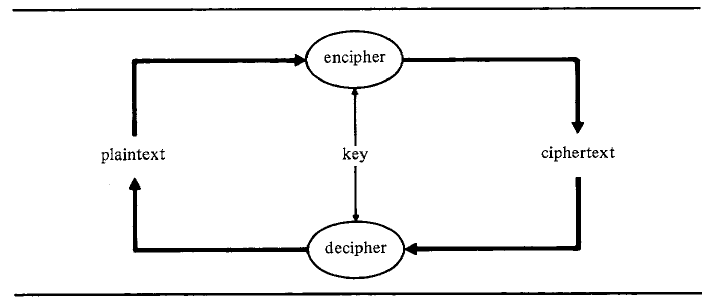
\includegraphics[width=0.8\textwidth]{./images/figExplicacionSistemaCripto}
	\caption{Descripción gráfica de un sistema criptográfico.}
	\label{figExplicacionSistemaCripto}
\end{figure}


En la actualidad se trabaja la criptografía sobre computadoras, es decir, cifrando y descrifrando bits, los cuales pueden tener diferentes significados, ya sea una imagen, un texto, un programa, etc. Esto significa que en la actualidad no se trabaja sobre caracteres del alfabeto o símbolos, sino más bien sobre 1's y 0's. Esto toma relevancia ya que al tener solo dos símbolos para cifrar, los algoritmos se vuelven más complejos por la falta de alternativas para sustituir un símbolo por otro.

Antiguamente la criptografía se basaba en caracteres que eran sustituidos o traspuestos por otros caracteres. Esto corresponde a cifrados de sustitución y de transposición, los cuales continúan siendo la base de la criptografía pero basado en los dos símbolos del sistema binario.

Como se explicó anteriormente el cifrado de sustitución se basa en tomar un caracter del texto plano y sustituirlo por otro caracter. Para descrifrar el texto cifrado simplemente se sustituyen de vuelta los caracteres y listo.

Según \cite{bruce} en la criptografía clásica existen 4 tipos de cifrado por sustitución:
\begin{itemize}
\item Cifrado de sustitución simple: Una sustitución de uno a uno entre cada caracter del texto plano y el texto cifrado.
Ejemplos de este tipo de sustitución son el famoso cifrado de César y el ROT13 utilizado en UNIX.

\item Cifrado de sustitución homofónico: Una sustición de uno a muchos. Un caracter del texto plano, por ejemplo A, puede ser sustituido por varios caracteres en el texto crifado, por ejemplo ``5'', ``13'', ``43''. Observe la Figura \ref{figExampleHomophonicCipher} donde se presenta una serie de posibles asignaciones de números a las letras del mensaje PLAIN PILOT y un posible texto cifrado haciendo uso de este tipo de cifrado.

\begin{figure}
	\centering
	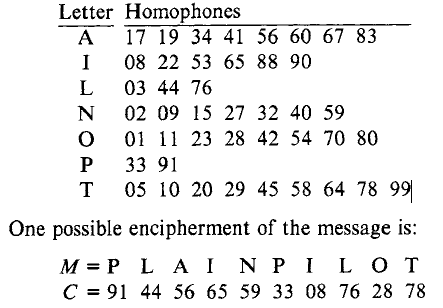
\includegraphics[width=0.6\textwidth]{./images/figExampleHomophonicCipher}
	\caption{Ejemplo de cifrado homofónico.}
	\label{figExampleHomophonicCipher}
\end{figure}


\item Cifrado de sustitución de poligrama: Una sustitución por bloques en donde se toma un bloque de caracteres del texto plano y se sustituye por su bloque equivalente en el texto cifrado. Por ejemplo si en el texto plano se tiene ``ABC'' se sustituye por ``SLL'' en el texto cifrado.

\item Cifrado de sustitución polialfabético: ????? 
\end{itemize}

La otra variedad de algoritmos son los de transposición, en este tipo de algoritmos criptográficos el texto plano se convierte en texto cifrado cuando el orden de los caracteres es cambiado bajo alguna norma. Un ejemplo moderno de este tipo de algoritmos es el \textit{rail-fence} donde el texto plano se reacomoda con la forma de una cerca como se observa en la Figura \ref{figExampleTranspositionCipher}. En este caso la llave del algoritmo sería la profundidad de la cerca, para efectos de este ejemplo es de 3.

\begin{figure}
	\centering
	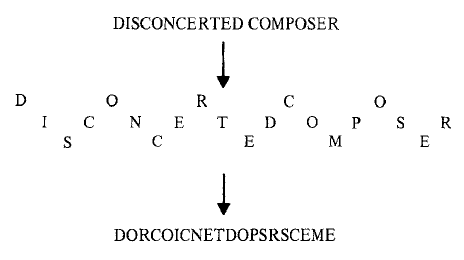
\includegraphics[width=0.65\textwidth]{./images/figExampleTranspositionCipher}
	\caption{Ejemplo de cifrado de transposición.}
	\label{figExampleTranspositionCipher}
\end{figure}


Actualmente en los algoritmos que se implementan en computadoras se combina tanto la tranposición como la sustitución. Por ejemplo se tiene el algoritmo RC5 (el cual se desarrollará más adelante en este proyecto), en donde se utiliza corrimientos o rotaciones a bits (tranposición) y sumas o XOR's (sustituciones) para cifrar el texto plano. Los algoritmos que se implementan en la criptografía moderna se dividen en dos categorías principales: simétricos y de llave pública (también llamados asimétricos \cite{denning}).


\section{Algoritmos criptográficos}
\subsection{Algoritmos simétricos}
\cite{bruce} da una muy buena analogía para explicar el concepto de un algoritmo simétrico. Piense en el algoritmo como una caja fuerte. La combinación de la caja fuerte vendría a ser la \textit{llave} del algoritmo. Note como en una caja fuerte cualquier persona con la combinación puede llegar, abrir la caja y poner o sacar documentos de la misma. En el caso de no conocer la combinación, se debe proceder a forzar la caja o probando todas las combinaciones posibles hasta hallar la correcta. Es decir en un algoritmo simétrico se cuenta con una llave única que funciona tanto para cifrar como para descrifrar los mensajes como se muestra en la Figura \ref{figSimmetricKeyAlgorithm}. La notación para el cifrado y descrifado en estos algoritmos se muestra en las Ecuaciones \eqref{eqCifradoSimetrico} y \eqref{eqDescifradoSimetrico}.
\begin{equation}\label{eqCifradoSimetrico}
E_K (M) = C
\end{equation}

\begin{equation}\label{eqDescifradoSimetrico}
D_K (C) = M
\end{equation}


\begin{figure}
	\centering
	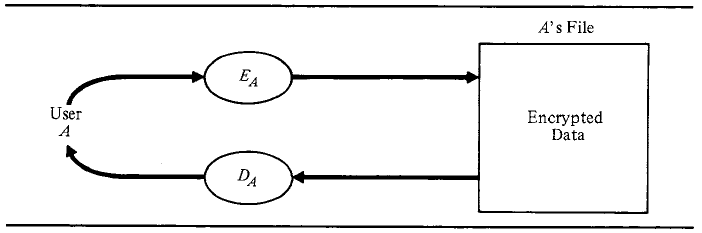
\includegraphics[width=0.9\textwidth]{./images/figSimmetricKeyAlgorithm}
	\caption{Descripción gráfica de una algoritmo de llave simétrica.}
	\label{figSimmetricKeyAlgorithm}
\end{figure}


Los algoritmos simétricos se dividen en 2 categorías (\cite{bruce}):

\begin{itemize}
\item Cifrado de bloque: Se cifra en bloques de bits ya sea \textit{bytes, words}, etc. Es decir cuando se va a proceder a cifrar un texto plano, se segmenta el texto en grupos de bits y estos son cifrados en conjunto. Se puede tomar como ejemplo el algoritmo \textit{Data Encryption Standart} (DES) el cual cifra sobre bloques de 64 bits. Otros ejemplos son:
\begin{itemize}
\item Lucifer.
\item LOKI.
\item 3-way.
\item RC5.
\item GOST.
\item IDEA.
\end{itemize}

\item Cifrado de \textit{Stream}: Es cuando se trabaja sobre un bit únicamente. Estos no son muy usuales en la actualidad ya que al trabajar en lenguaje binario solo se cuenta con 2 símbolos y si se cifra únicamente un bit no existen muchas posibilidades para sustituir o transposicionar.
Ejemplos de estos algoritmos pueden ser:
\begin{itemize}
\item RC4.
\item SEAL.
\item WAKE.
\end{itemize}
\end{itemize}

Según (\cite{bruce}) los criptosistemas simétricos en la red afrontan los siguientes problemas
\begin{itemize}
\item Distribución de la llave: La llave se debe mantener en secreto. Esto en la actualidad es una tarea demasiado díficil de lograr porque la llave debe ser conocida para el cifrado y descifrado (emisores y receptores) entonces para establecer una comunicación segura el primer paso debe ser entregar la llave de forma segura, lo cual en una red de computadoras se puede tornar una tarea prácticamente imposible de realizar. La única solución sería entregar las llaves mediantes un servicio de \textit{courier} o similares e igualmente se corren riesgos. 

\item Compromiso de seguridad: Si la llave es conocida por un tercero, si este intercepta el tráfico de información, todas las comunicaciones serán descifradas fácilmente.

\item Comunicaciones aisladas: En el caso de que cada usuario de una red se desee comunicar secretamente por separado con todos los otros usuarios haciendo uso del mismo criptosistema, se debe utilizar una llave diferente para cada comunicación. Así para una red de N usuarios se requieren $N(N - 1)/2$ llaves. A primera vista esto no parece tan importante por ejemplo para 10 usuarios, se necesitan 45 llaves lo cual está bien, pero para 100 usuarios se necesitarían 4950 llaves que se tienen que distribuir de forma secreta.
\end{itemize}



\subsection{Algoritmos de llave pública}
Nuevamente \cite{bruce} nos ofrece una excelente analogía para explicar, en este caso, los algoritmos de llave pública. Tenemos un \textit{mailbox}, donde cualquier persona puede poner un mensaje adentro pero ÚNICAMENTE el dueño puede abrirlo para sacar y leer los mensajes.
\newline
\newline
En los algoritmos de llave pública los emisores hacen uso de una llave para cifrar los mensajes que desean enviar pero estos mensajes pueden ser descrifrados únicamente si se tiene la llave para descifrar mensajes (que es diferente de la llave para cifrar), la cual el receptor la tendrá bien resguardada. En la Figura \ref{figPublicKeyAlgorithm} se muestra el diagrama básico de un algoritmo de llave pública. Ejemplos de estos algoritmos pueden ser:
\begin{itemize}
\item RSA
\item Pohlig-Hellman
\item Rabin
\item ElGamal
\end{itemize}

\begin{figure}
	\centering
	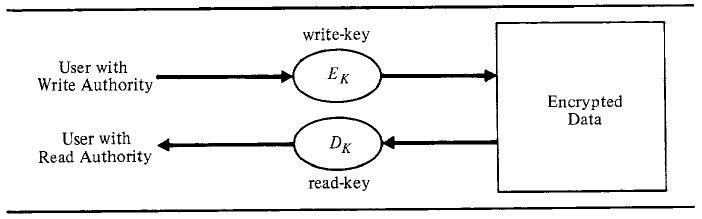
\includegraphics[width=0.65\textwidth]{./images/figPublicKeyAlgorithm}
	\caption{Descripción gráfica de una algoritmo de llave pública.}
	\label{figPublicKeyAlgorithm}
\end{figure}

Estos algoritmos sientan su base matemática en funciones llamadas \textit{one-way} en donde al aplicarle una función a una variable, la variable no puede retornar a su valor original de ninguna manera, es decir la función no tiene una inversa. 

Según \cite{bruce} existen funciones \textit{one-way} con una ``puerta trasera'' donde se puede retornar a la variable original conociendo ciertos parámetros, este tipo de funciones son las que se implementan en algoritmos de llave pública. Los algoritmos dominantes de esta rama se basan en la dificultad de factorizar números grandes que son el resultado de multiplicar dos números primos grandes como también se basan en el \textit{Discrete Logarithm Problem}.

En estos algoritmos no es posible a partir de la llave para cifrar obtener la llave para descrifrar. Esto permite que la llave para cifrar se pueda hacer pública, por lo cual recibe el nombre de llave pública y la llave para descrifrar se denomina llave privada. La notación para estos algoritmos corresponde a la de las Ecuaciones \eqref{eqCifradoPublico} y \eqref{eqDescfiradoPublico}
\begin{equation} \label{eqCifradoPublico}
E_{K_x} (M) = C
\end{equation}
\begin{equation} \label{eqDescfiradoPublico}
D_{K_y} (C) = M
\end{equation}

El objetivo de utilizar cifrado de llave pública se basa en:
\begin{itemize}
\item Receptor y emisor acuerdan un sistema criptográfico.
\item El receptor entrega al emisor su llave pública.
\item El emisor cifra el texto plano haciendo uso de la llave pública entregada y el sistema acordado.
\item El emisor envía el texto cifrado.
\item El receptor descrifa el texto cifrado haciendo uso de la llave privada.
\end{itemize}

De esta manera no hay forma que fisgones logren descrifrar el mensaje aunque obtengan la llave pública, así el receptor se asegura que las comunicaciones van a ser mucho más seguras ya que el emisor deja de tener la llave para descifrar y no puede brindarsela a nadie o que le sea robada a este. Para la implementación de un criptosistema que hace uso de algoritmos de llave pública, lo que se hace es que en la red se tiene una base de datos donde se registra el usuario y su respectiva llave pública, así cuando un usuario se desea comunicar con otro, va a la base de datos, busca al usuario y su llave pública, cifra el mensaje con la misma y se la envía. Esto solventa los problemas que presentaba anteriormente los algoritmos simétricos, ya que no es necesario transmitir de forma secreta llaves para poder realizar comunicaciones y para que diferentes usuarios se comuniquen de forma secreta entre si no es necesario el uso de diferentes llaves por cada enlace de comunicación. 

Algunos usos de estos algoritmos en la actualidad son:
\begin{itemize}
\item Llave maestra para el sistema de pago digital de un banco.
\item La clave que utiliza un gobierno para certificar sus visas o pasaportes.
\item La firma digital es un notario público.
\end{itemize} 

\subsection{Criptosistemas híbridos}
Los beneficios que conlleva utilizar algoritmos de llave pública son grandes pero se pagan a un precio muy alto: tiempo de procesamiento. Según \cite{bruce} el tiempo de procesamiento del RSA con respecto al del DES es de alrededor de 1000 mil veces más lento. 

En un mundo donde la velocidad es una clave fundamental en las comunicaciones se propuso la siguiente solución. Ya que los algoritmos simétricos tienen la debilidad de comunicar la llave antes de comenzar la comunicación pero son mucho más rápidos, y que los algoritmos de llave pública ostentan una mejor sistema para comunicarse en la red secretamente pero son muy lentos, se decidió utilizar ambos. La llave del algoritmo simétrico es encriptada con un algoritmo de llave pública para transmistirse en la red sin comprometerla y posterior a esto se realizan las comunicaciones con el algoritmo simétrico para obtener una mejor velocidad de comunicación. Se puede ver el protocolo de la siguiente manera (\cite{bruce}):
\begin{itemize}
\item El receptor envía su llave pública al emisor.
\item El emisor genera una llave de sesión\footnote{A common cryptographic technique is to encrypt each individual conversation with a separate key. This is called a session key, because it is used for only one
particular communications session. As discussed in Section 8.5, session keys
are useful because they only exist for the duration of the communication. How
this common session key gets into the hands of the conversants can be a
complicated matter.}, la cifra y se la envía al receptor usando la llave pública que le fue dada.
\item El receptor descrifra la llave de sesión usando su llave privada.
\item Ahora ambos pueden comunicarse de forma secreta con la llave de sesión con un criptosistema simétrico.
\end{itemize}





\section{Seguridad en algoritmos criptográficos}
Como parte de la investigación previa para este proyecto no podemos dejar de lado la otra cara de la moneda, el criptoanálisis. La ciencia que abarca la criptografía y el criptoanálisis es conocida como criptología (\cite{denning}). Claramente el objetivo de la criptografía es mantener un mensaje en secreto de terceros, pues el criptoanálisis según (\cite{raeAnalisis}) es el ``arte de descifrar criptogramas'', así es como los terceros buscan inmiscuirse en las comunicaciones secretas sin tener un acceso a la llave.  

Según \cite{bruce}, el criptógrafo al diseñar su algoritmo debe asumir que el criptoanalista puede tener un acceso completo a las comunicaciones entre emisor y receptor y al algoritmo que implementa el criptosistema, así toda la seguridad del criptosistema debe residir en la llave.

La acción en la que un criptoanalista atenta contra un criptosistema es denominada \textit{ataque}. Según \cite{bruce} y \cite{denning} los principales tipos de ataques son:
\begin{itemize}

\item \textit{Ciphertext-only}: El criptoanalista debe obtener la llave a partir de varios textos cifrados. Debe conocer el tema tratado de las comunicaciones que está interviniendo (lo cual es obvio, ya que sino para qué está interviniendo las comunicaciones) entonces puede saber de forma previa que ciertas cosas que puede contener el texto plano.

\item \textit{Known-plaintext}: El criptoanalista tiene acceso a ciertos textos planos y sus respectivos textos cifrados. A partir de estos debe deducir la llave o debe generar un algoritmo de descifrado equivalente al diseñado por el criptográfo.

\item \textit{Chosen-plaintext}: El criptoanalista puede obtener el texto cifrado de un texto plano que él seleccione, esto es mucho más poderoso porque puede encriptar mensajes que den más información acerca de la llave por ejemplo. Un sistema de bases de datos es vulnerable a este tipo de ataques debido a que los usuarios pueden agregar elementos a la base de datos y ver el resultado del texto cifrado en la misma. Nuevamente su tarea es obtener la llave o generar un algoritmo de descifrado equivalente.

\item \textit{Chosen-ciphertext}: Este tipo de ataque se da en algoritmos de llave pública, en donde el criptoanalista tiene acceso al texto cifrado que va a ser descifrado y al texto plano. Es decir tiene una ``caja negra'' donde la entrada es el texto cifrado y la salida el texto plano. El objetivo es obtener la llave a partir de estos recursos.

\item \textit{Chosen-key}: El criptoanalista tiene conocimiento sobre la relación entre las diferentes llaves.

\item \textit{Rubber-hose}: El criptoanalista amenaza, extorsiona, chantajea u obtiene de alguna forma la llave sin ningún tiempo.
\end{itemize}


Otro ejemplo es que los algoritmos de llave pública son vulnerables a ataques de tipo \textit{chosen-plaintext}. Tome por ejemplo M como un texto plano del espacio $M$ de posibles mensajes. La tarea de un criptoanalista es tomar todos $\text{M} \epsilon M$ y cifrarlos para obtener todos los posibles $\text{C} \epsilon C$. De esta manera solo debe interceptar las comunicaciones que desea y comparar sus valores de texto cifrado con los que intercepta para descifrar las comunicaciones. Note que el criptoanalista no pudo obtener la llave pero si logró descrifrar las comunicaciones.


\subsection{Tamaño de la llave}
Como se mencionó anteriormente la seguridad de un buen algoritmo depende de su llave. Asumiendo que se tiene una seguridad del algoritmo perfecta, la única forma de quebrar el criptosistema sería mediante un ataque de fuerza bruta, el cual es un tipo de ataque \textit{known-plaintext}, para obtener la llave. 

Analizando el tamaño de la llave, si se tuviera una de $2^8$ bits, probando las 256 posibilidades se obtendría la llave, lo cual equivale a unos cuantos segundos de procesamiento en una computadora. Para $2^{64}$ bits tenemos $1.8446744^{19}$ posibles llaves, lo cual tomaría con los recursos computacionales de una supercomputadora alrededor de 585,000 años. Para una llave de 2048, con un billón de intentos por segundo en computadoras en paralelo se necesitarían 10597 años para encontrar la llave \cite{bruce}. 


Entonces ¿Porqué no hacer un algoritmo con una llave muy grande?. La respuesta es porque conforme aumenta el tamaño de la llave, se paga en tiempo de procesamiento. Así se debe obtener un balance donde la llave sea lo suficientemente grande para que sea el algoritmo sea seguro, pero lo suficientemente pequeña para que el tiempo de procesamiento sea bueno (\cite{bruce}).

Comparar el nivel de seguridad ante un ataque de fuerza bruta de un algoritmo simétrico y uno de llave pública con llaves del mismo tamaño no es posible, pero la Figura \ref{figVariacionLlaves} muestra una tabla con equivalentes realizados empíricamente por \cite{bruce} sobre tamaños de llaves que dan un nivel de seguridad equivalente para los dos tipos de algoritmos, esto nos indica que no es recomendable comparar algoritmos de distintas ramas entre sí.

\begin{figure}
	\centering
	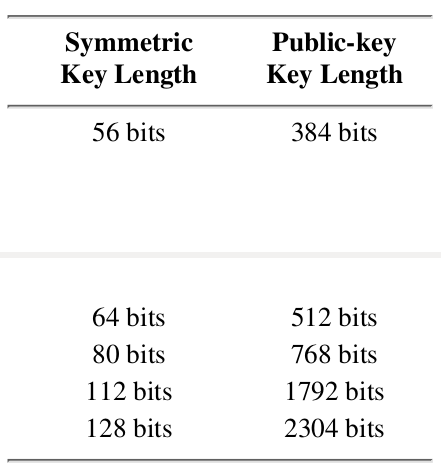
\includegraphics[width=0.65\textwidth]{./images/figVariacionLlaves}
	\caption{Comparación del tamaño de llaves en algoritmos simétricos y asimétricos.}
	\label{figVariacionLlaves}
\end{figure}

\subsection{Manejo de las llaves}
Se puede tener un algoritmo extremadamente robusto, veloz y con un tamaño de llave perfecto, pero si un atacante puede obtener la llave por algún medio el algoritmo es completamente inútil. De ahí la gran importancia de como manejar las llaves.

Al ser esto tan importante existen ciertas maneras de generar llaves:
\begin{itemize}
\item Ingresada por el usuario: El usuario elige una llave y esa es la que se va a utilizar. Este método es sumamente inseguro
debido a que gran cantidad de contraseñas se repiten, o son datos personales del usuario como su número de celular o similares.
Por tanto se pueden realizar \textit{ataques de diccionario} donde las primeras llaves que se prueban son las mencionadas
anteriormente.

\item Random keys: Es un muy buen método para generar llaves, consiste en utilizar un programa que genere la llave, es ventajoso
ya que es robusto ante ataques de diccionario pero presenta el problema que la llave es difícil de recordar y posiblemente se olvide.

\item pass phrases: Es una combinación de ambos, el usuario escribe una contraseña fácil de recordar y después
hace uso de un one-way has function para convertir esta llave en una llave random de tamaño arbitrario.
\end{itemize}





\section{Escogencia de los algoritmos a implementar}
En un principio el objetivo de este proyecto era realizar una comparación con las métricas descritas en la Introducción sobre un algoritmo simétrico y un algoritmo de llave pública, posterior a la realización del marco teórico se llegó a la conclusión de que realizar este análisis no iba a ser para nada justo debido mayoritariamente a tres razones:
\begin{itemize}
\item El tiempo de procesamiento: Como se menciona anteriormente los algoritmos de llave pública consumen mucho más tiempo realizando el cifrado y descifrado que un algoritmo de llave simétrica.
\item La formas en las que estos algoritmos son diseñados producen falencias en seguridad distintas por lo cual analizar comparativamente no sería tan interesante.
\item Los algoritmos realizan el proceso de cifrado de maneras muy diferentes: En el caso de los algoritmos simétricos son basados en transposición y sustitución que trabajan en su mayoría con XOR's, sumas y corrimientos. En cambio los algoritmos de llave pública trabajan  basados en la multiplicación de números primos y \textit{Discrete Logarithm Problem} donde ocurren muchas multiplicaciones y sumas. Esto produce un consumo de recursos muy diferente entre ambos tipos.
\end{itemize}

Bajo el criterio que ambos algoritmos tuvieran características similares para poder ser analizados comparativamente y que fueran fáciles de implementar a nivel de hardware se optó por comparar dos algoritmos simétricos, específicamente el RC5 y el IDEA los cuales están basados en redes de Feistel\footnote{Feistel Networks
Most block algorithms are Feistel networks. This idea dates from the early
1970s [552,553]. Take a block of length n and divide it into two halves of
length n/2: L and R. Of course, n must be even. You can define an iterated
block cipher where the output of the ith round is determined from the output of
the previous round:
Li = Ri - 1
Ri = Li - 1  f(Ri - 1,Ki)
Ki is the subkey used in the ith round and f is an arbitrary round function.
You’ve seen this concept in DES, Lucifer, FEAL, Khufu, Khafre, LOKI,
GOST, CAST, Blowfish, and others. Why is it such a big deal? The function is
guaranteed to be reversible. Because XOR is used to combine the left half with
the output of the round function, it is necessarily true that
Li - 1  f(Ri - 1,Ki)  f(Ri - 1,Ki) = Li - 1
A cipher that uses this construction is guaranteed to be invertible as long as the
inputs to f in each round can be reconstructed. It doesn’t matter what f is; f
need not be invertible. We can design f to be as complicated as we please, and
we don’t have to implement two different algorithms—one for encryption and
another for decryption. The structure of a Feistel network takes care of all this
automatically.
} y por tanto comparten características de diseño para que la comparación sea un poco más justa.



\section{Descripción de los algoritmos a implementar}
\subsection{RC5}


\subsection{IDEA o LUCIFER o FEAL}






\section{Características de un FPGA}




	
	%desarrollo
	%\chapter{Resultados y análisis}
En esta capítulo se va a mostrar y analizar los resultados de realizar la implementación de los algoritmos criptográficos RC5 y TEA.
Primero se dan resultados y análisis individuales, para posteriomente realizar el análisis comparativo.

Las síntesis e implementaciones se llevaron a cabo haciendo uso de la herramienta de desarrollo \textit{Vivado Design Suite} de \textit{Xillinx} bajo la licencia gratuita \textit{WEBPack}. Se hizo utilizó como objetivo de implementación la tarjeta xc7k70tfbv676-1 de la familia de FPGAs \textit{Kintex-7}. En la Tabla \ref{tabRecursosFPGA} se muestran todos los recursos disponibles de la misma. 

\begin{table}[htbp]
  \centering
  \caption{Recursos disponible para el FPGA Kintex-7 xc7k70tfbv676-1 de Xillinx.}
    \begin{tabular}{lr}
    \toprule
    Componente & Cantidad Disponible\\
    \midrule
	Slices & 10250\\
	Slice LUTs & 41000\\
	Slice Registers & 82000\\
	Block RAM & 135\\
	DSPs & 240\\
	I/O ports & 300\\
    \bottomrule
    \end{tabular}%
  \label{tabRecursosFPGA}%
\end{table}%

Para poder obtener las métricas que se analizan se utilizaron los reportes de temporización y utilización que la herramienta ofrece al finalizar el proceso de implementación. Se guardaron estos archivos después de cada sintesís e implementación y se utilizó un \textit{script} de Python para extraer los datos deseados y escribirlos a un archivo CSV (\textit{Comma Separated Values}) para poder abrir el mismo haciendo uso de \textit{Excel} para graficar las diferentes métricas haciendo uso de tablas pivote para un análisis más eficiente.


Cabe aclarar que aunque en un principio no se iba a tomar en cuenta el análisis de temporización, específicamente la frecuencia máxima de reloj, la misma fue agregada a la lista de métricas a analizar debido a que en la implementación realizada la frecuencia máxima de reloj afecta directamente el tiempo de procesamiento para cifrar y descifrar datos y por tanto es una métrica muy importante a analizar. Agregado a esto se puede destacar el hecho de que igualmente a causa de la implementación el variar la cantidad de rondas que cifran o descifran los datos no afectan de ninguna manera la cantidad de recursos del FPGA y solo afectan el tiempo de procesamiento total de cifrado o descifrado.


Otro aspecto importante es que se asumió que los módulos \textit{top} de los algoritmos son módulos que serán parte de un dispositivo más grande (por ejemplo un procesador) y por tanto que ese dispositivo hará uso de tanto los módulos de cifrado y descifrado, así los módulos serán sintetizados e implementados simúltaneamente para cada algoritmo, ya que el análisis de ambos módulos tendrá más valor que el de los módulos por separado. Particularmente para el algoritmo RC5 se hizo que los módulos de cifrado y descifrado compartan el módulo que se encarga de la expansión de llave (\textit{keyExpander} en las Figuras \ref{figCipherBlockDiagram} y \ref{figDecipherBlockDiagram}) esto con la finalidad de consumir la menor cantidad de recursos y hacer lo más óptimo posible el diseño.


Un problema al que se enfrentó al implementar los algoritmos en el FPGA es que la cantidad de salidas y entradas del diseño era muy grande para que el mismo fuera implementable en el FPGA. La solución a esto corresponde a un módulo para serializar y deserializar las entradas y salidas pero el mismo no fue implementado ya que no era uno de los objetivos del proyecto, además de que se consideró innecesario ya que, como se indicó anteriormente, estos algoritmos formarían parte de un dispositivo más grande que ya contará con este módulo. Así para poder implementar el diseño simplemente se pusieron dos puertos, uno de entrada y otro de salida, ambos del tamaño de la palabra y las señales de control de los módulos.

\section{Resultados y análisis del algoritmo TEA} \label{resultadosAnalisisTEA}
Inicialmente se corroboró que el algoritmo funcionara correctamente, esto se logró comparando los resultados de texto cifrado y descifrado con el código en C que se encuentra en los Listados \ref{lstCipherTEA} y \ref{lstDecipherTEA}\footnote{El código para verificar fue ligeramente diferente al de los listados debido a que se tuvo que ajustar para poder variar el tamaño de palabra.}. La Tabla \ref{tabSimTEA} muestra el resultado de cifrado y descifrado al simular con diferentes tamaños de palabra para 32 rondas de cifrado/descifrado. Además la tabla en la columna \textit{layout} indica un número de figura al cual está ligado la implementación para el tamaño de palabra. Este \textit{layout} corresponde al dado por la herramienta de desarrollo para observar la distribución de recursos en el circuito. Además el camino resaltado en blanco en cada \textit{layout} corresponde al \textit{critical path} de cada implementación.

\begin{table}[htbp]
  \centering
  \caption{Resultados de simulación del TEA para diferentes tamaños de palabra.}
    \begin{tabular}{lrrr}
    \toprule
	\begin{tabular}[c]{@{}l@{}}Tamaño\\de palabra\\(bits)\end{tabular} & Texto plano (hex) & Texto cifrado (hex) & Figura \textit{layout} \\
    \midrule
	8 & 0d8d & aba7 & \ref{fig8_32_layout} \\
	\midrule
	16 & 7b0d998d & 829789bc &  \ref{fig16_32_layout} \\
	\midrule
	32 & 3d45f7a7235fcb21 & f5509056d5db9e6a & \ref{fig32_32_layout} \\
	\midrule
	64 & \begin{tabular}[c]{@{}l@{}}0000000006b97b0d\\0000000046df998d\end{tabular}  & \begin{tabular}[c]{@{}l@{}}0d85f88a9ef595ff\\4810210e9e2a4f5e\end{tabular} & \ref{fig64_32_layout} \\
	\midrule
	128 & \begin{tabular}[c]{@{}l@{}}3ca67c8e15890877\\6dcc3a7b41cb88e6\\9a34483d3b1a68a4\\1235130bf207ee95\end{tabular} & \begin{tabular}[c]{@{}l@{}}c0144f6419ce0203\\dbee17be33c2bf5c\\87b4dc12f9cbe22f\\f2f826efc585fa46\end{tabular} & \ref{fig128_32_layout} \\
    \bottomrule
    \end{tabular}%
  \label{tabSimTEA}%
\end{table}%


\begin{figure}[H]
	\centering
	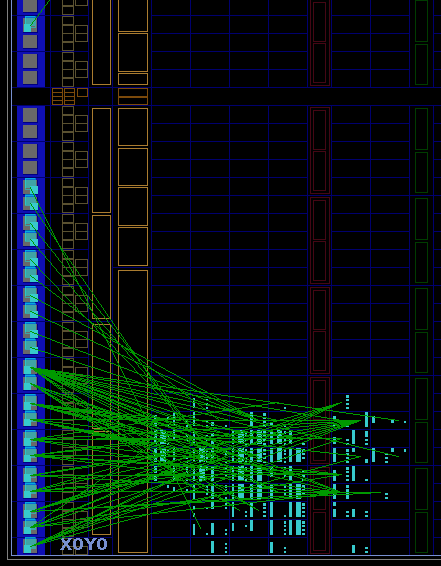
\includegraphics[width=0.9\textwidth]{./images/fig8_32_layout}
	\caption{\textit{Layout} de la implementación del algoritmo TEA de 8 bits de tamaño de palabra y 32 rondas de cifrado/descifrado.}
	\label{fig8_32_layout}
\end{figure}

\begin{figure}[H]
	\centering
	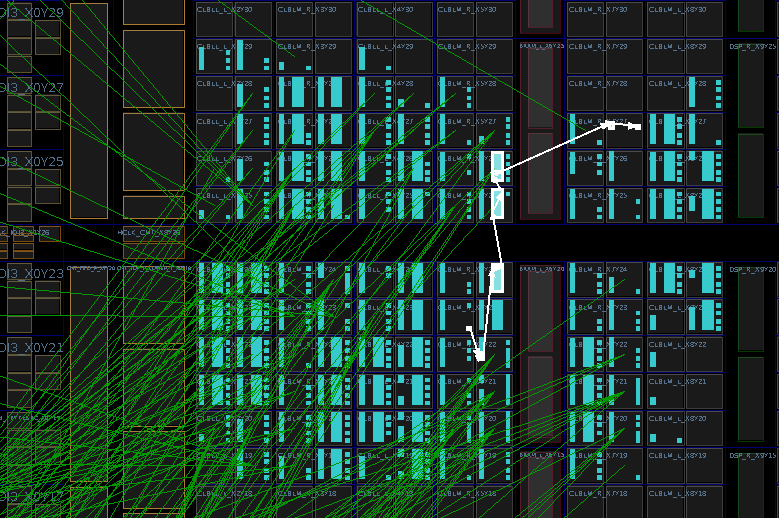
\includegraphics[width=0.9\textwidth]{./images/fig16_32_layout}
	\caption{\textit{Layout} de la implementación del algoritmo TEA de 16 bits de tamaño de palabra y 32 rondas de cifrado/descifrado.}
	\label{fig16_32_layout}
\end{figure}

\begin{figure}[H]
	\centering
	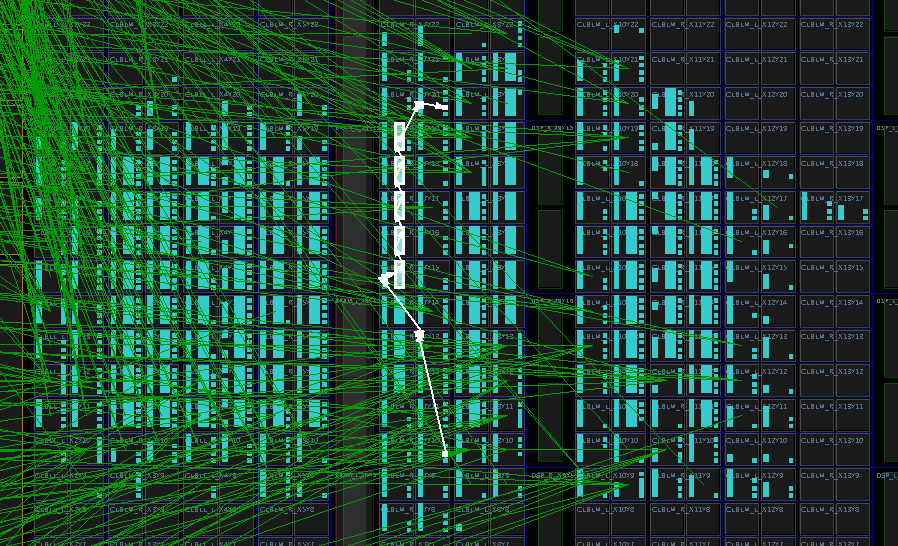
\includegraphics[width=0.9\textwidth]{./images/fig32_32_layout}
	\caption{\textit{Layout} de la implementación del algoritmo TEA de 32 bits de tamaño de palabra y 32 rondas de cifrado/descifrado.}
	\label{fig32_32_layout}
\end{figure}

\begin{figure}[H]
	\centering
	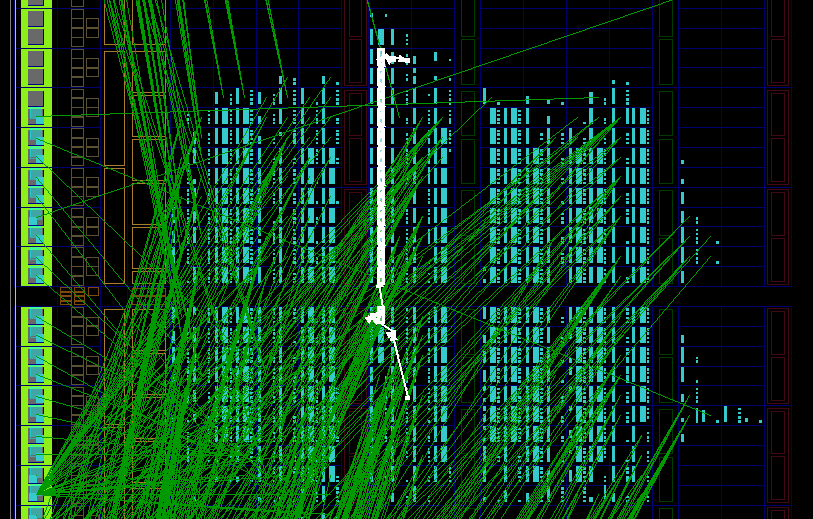
\includegraphics[width=0.9\textwidth]{./images/fig64_32_layout}
	\caption{\textit{Layout} de la implementación del algoritmo TEA de 64 bits de tamaño de palabra y 32 rondas de cifrado/descifrado.}
	\label{fig64_32_layout}
\end{figure}

\begin{figure}[H]
	\centering
	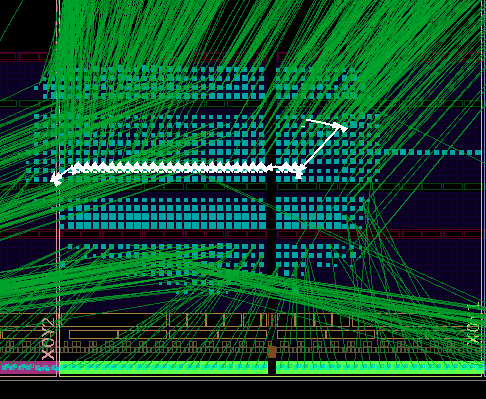
\includegraphics[width=0.9\textwidth]{./images/fig128_32_layout}
	\caption{\textit{Layout} de la implementación del algoritmo TEA de 128 bits de tamaño de palabra y 32 rondas de cifrado/descifrado.}
	\label{fig128_32_layout}
\end{figure}


En el caso de este algoritmo los parámetros que se variaron y cómo se variaron se muestran en la Tabla \ref{tabVariacionTEA} donde se fijó la cantidad de rondas en el valor nominal del algoritmo, 32 rondas de cifrado/descifrado\footnote{Para tamaños de palabra mayores a 128 se consideró innecesario el análisis debido a que ya un tamaño de palabra tan grande no es óptimo de utilizar bajo ninguna circunstancia.}.  Además en esa misma tabla se muestra el consumo de recursos del FPGA al variar esos parámetros. Note en los Listados \ref{lstCipherTEA} y \ref{lstDecipherTEA} como por el algoritmo no es posible variar independientemente el tamaño de la llave del tamaño de la palabra a cifrar y por tanto no es posible realizar un análisis independiente del análisis de la variación del tamaño de llave y como afecta los recursos del FPGA. 

% Table generated by Excel2LaTeX from sheet 'datos'
\begin{table}[htbp]
  \centering
  \caption{Variación de parámetros del algoritmo TEA y consumo de recursos del FPGA.}
    \begin{tabular}{rrrrrrr}
    \toprule
    \begin{tabular}[c]{@{}l@{}}Tamaño\\palabra\\(bits)\end{tabular}  & \begin{tabular}[c]{@{}l@{}}Tamaño\\llave\\(bits)\end{tabular} & \begin{tabular}[c]{@{}l@{}}LUT as\\Logic\end{tabular}  & Slice L & Slice M & \begin{tabular}[c]{@{}l@{}}Slice\\Registers\end{tabular} & \begin{tabular}[c]{@{}l@{}}Frecuencia \\máx. (MHz)\end{tabular}   \\
    \midrule
    8     & 32    & 217   & 45    & 27    & 176   & 434,783 \\
    16    & 64    & 383   & 74    & 38    & 328   & 392,157 \\
    32    & 128   & 737   & 133   & 90    & 632   & 338,983 \\
    64    & 256   & 1439  & 243   & 179   & 1240  & 303,030 \\
    128   & 512   & 2841  & 439   & 357   & 2456  & 217,391 \\

    \bottomrule
    \end{tabular}%
  \label{tabVariacionTEA}%
\end{table}%
		
De la Tabla \ref{tabVariacionTEA} se pueden extraer las gráficas que se muestran en las Figuras \ref{figSlicesTEA}, \ref{figSliceRegsLutsTEA} y \ref{figFrecuenciasTEA}.

La Figura \ref{figSlicesTEA} muestra como varía la cantidad de \textit{slices} tanto de tipo L como M conforme el tamaño de palabra varía. La Figura \ref{figSliceRegsLutsTEA} muestra como varía la cantidad de \textit{slice registers} y LUTs al variar el tamaño de la palabra. Note como después de variar la palabra de 32 bits a 64 bits la cantidad de recursos comienza a aumentar mostrando un comportamiento exponencial. Además la relación de ambas gráficas es la esperada ya que muestran la misma tendencia debido a que los \textit{slices} se encuentran compuestos por registros y LUTs.

\begin{figure}[H]
	\centering
	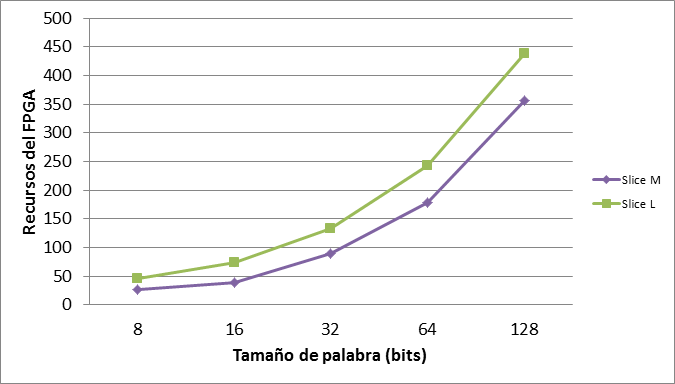
\includegraphics[width=0.9\textwidth]{./images/figSlicesTEA}
	\caption{Gráfica de variación de \textit{slice L} y \textit{slice M} contra la variación del tamaño de palabra en bits al implementar el algoritmo TEA.}
	\label{figSlicesTEA}
\end{figure}
\begin{figure}[H]
	\centering
	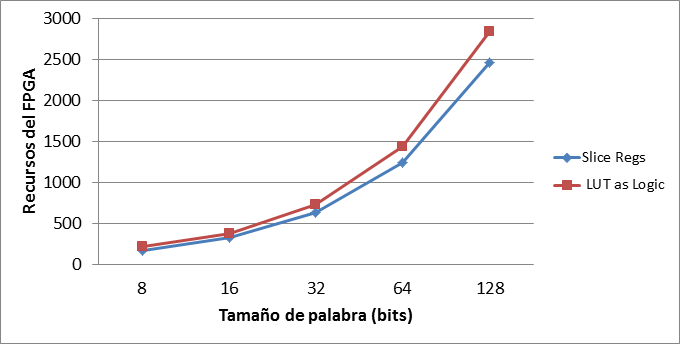
\includegraphics[width=0.9\textwidth]{./images/figSliceRegsLutsTEA}
	\caption{Gráfica de variación de \textit{slice registers} y LUTs contra la variación del tamaño de palabra en bits al implementar el algoritmo TEA.}
	\label{figSliceRegsLutsTEA}
\end{figure}

La Figura \ref{figFrecuenciasTEA} muestra la variación de la frecuencia máxima de reloj conforme el tamaño de palabra varía. El comportamiento es el esperado hasta cierto punto, ya que la frecuencia de reloj disminuye pero era esperado que la misma disminuyera de forma exponencial al igual que el consumo de recursos iba aumentando. Esto puede deberse a que la herramienta de desarrollo optimiza el proceso de \textit{place \& route} para lograr la mejor respuesta del diseño.

\begin{figure}[H]
	\centering
	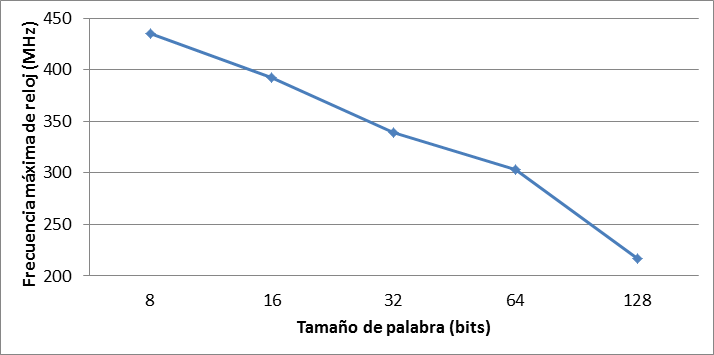
\includegraphics[width=0.9\textwidth]{./images/figFrecuenciasTEA}
	\caption{Gráfica de variación de la frecuencia máxima de reloj contra la variación del tamaño de palabra en bits al implementar el algoritmo TEA.}
	\label{figFrecuenciasTEA}
\end{figure}	
	
Finalmente los datos de la Tabla \ref{tabVariacionTEA} fueron normalizados respecto al valor mínimo de cada columna (por ejemplo 217 en la columna \textit{LUT as Logic}) con la finalidad de dar un análisis más acertado sobre cual sería el tamaño de palabra más conveniente a utilizar para este algoritmo. Los datos normalizados se muestran en la Tabla \ref{tabNormalizadoTEA} y se reflejan en la gráfica de la Figura \ref{figNormalizadoTEA}.

% Table generated by Excel2LaTeX from sheet 'datos'
\begin{table}[htbp]
  \centering
  \caption{Variación de parámetros del algoritmo TEA y consumo de recursos del FPGA normalizados.}
    \begin{tabular}{rrrrrrr}
    \toprule
    \begin{tabular}[c]{@{}l@{}}Tamaño\\palabra\\(bits)\end{tabular}  & \begin{tabular}[c]{@{}l@{}}Tamaño\\llave\\(bits)\end{tabular} & \begin{tabular}[c]{@{}l@{}}LUT as\\Logic\end{tabular}  & Slice L & Slice M & \begin{tabular}[c]{@{}l@{}}Slice\\Registers\end{tabular} & \begin{tabular}[c]{@{}l@{}}Frecuencia \\máx. reloj\end{tabular}   \\
    \midrule
    8     & 32    & 1,00  & 1,00  & 1,00  & 1,00  & 2,00 \\
    16    & 64    & 1,76  & 1,64  & 1,41  & 1,86  & 1,80 \\
    32    & 128   & 3,40  & 2,96  & 3,33  & 3,59  & 1,56 \\
    64    & 256   & 6,63  & 5,40  & 6,63  & 7,05  & 1,39 \\
    128   & 512   & 13,09 & 9,76  & 13,22 & 13,95 & 1,00 \\
    \bottomrule
    \end{tabular}%
  \label{tabNormalizadoTEA}%
\end{table}%

\begin{figure}[H]
	\centering
	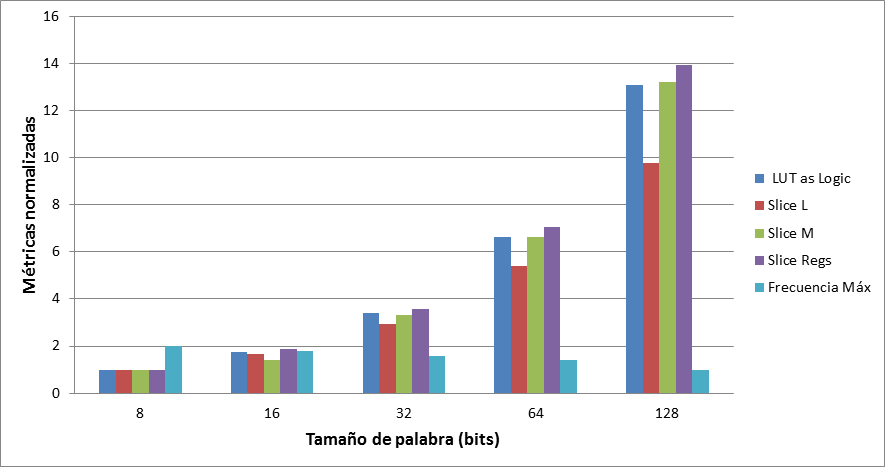
\includegraphics[width=1\textwidth]{./images/figNormalizadoTEA}
	\caption{Gráfica de consumo de recursos y frecuencia máxima (normalizados respecto al valor mínimo) del FPGA contra la variación del tamaño de palabra en bits al implementar el algoritmo TEA.}
	\label{figNormalizadoTEA}
\end{figure}
	
	
Note nuevamente como los recursos muestran el comportamiento exponencial descrito en las otras gráficas, pero como esta gráfica en particular los datos se muestran normalizados, el análisis se puede realizar de manera global.

Analizando la gráfica de la Figura \ref{figNormalizadoTEA} el comportamiento esperado es que al duplicar el tamaño de palabra se debe aumentar la cantidad de recursos consumidos en el FPGA al doble, así como reducir a la mitad la frecuencia máxima de reloj. Contrario a los resultados esperados se observa como conforme se varía el tamaño de palabra los recursos tienden ser menores al doble y la proporción se aleja cada vez más de ser el doble. Esto se puede deber nuevamente a la herramienta de desarrollo que puede optimizar el diseño \textcolor{red}{DE QUE MANERA??????????}. En el caso de la frecuencia máxima de reloj se observa como hasta que la palabra llega a ser de 128 bits se obtiene la frecuencia de la mitad de la frecuencia para el tamaño de palabra de 8 bits, esto se debe nuevamente (y como se explicó anteriormente en el análisis de la Figura \ref{figFrecuenciasTEA}) a la herramienta de desarrollo.


Finalmente bajo los análisis dados anteriormente se puede concluir que el tamaño de palabra ideal podría ser cualquiera menor a 32 bits. Las razones de esto son las siguientes:

\begin{itemize}
\item El tamaño de palabra de 32 bits, implica una entrada de texto plano de 64 bits, la cual se ajusta perfectamente al tamaño de palabra actual de la mayoría de procesadores de computadoras personales. También existen muchos microcontroladores con procesadores con tamaños de palabra de 32 bits o 16 bits, lo cual indicaría para el algoritmo tamaños de palabra de 8 bits o 16 bits. El beneficio de ``acoplar'' de alguna manera las entradas y salidas del algoritmo a las entradas y salidas del procesador es que en el cifrado puede procesar inmediatamente la información conforme esta sale del procesador y en el caso del descifrado es que puede entregar inmediamente al procesador la información descifrada y continuar descifrando datos.\footnote{Inclusive existen microcontroladores con procesadores de 8 bits por ejemplo el HC 08 de Freescale (\url{http://www.freescale.com/products/more-processors/8-bit-mcus/hc08:HC08FAMILY?cof=0&am=0}). Entonces sería válido realizar un análisis para 4 bits de tamaño de palabra del algoritmo.}

\item Las frecuencias máximas de reloj a las que trabajan esas implementaciones son mucho mayores que en las implementaciones de palabras de mayor tamaño.

\item Aunque puede ocurrir una disminución en el nivel de seguridad del algoritmo al trabajar con palabras más pequeñas, esta se puede aumentar aumentando la cantidad de rondas de cifrado y al trabajar a una frecuencia más alta el impacto en el desempeño no es tanto.

\item Se ahorra una gran cantidad de recursos en el FPGA el cual se traduce directamente en costos de producción.
\end{itemize}

\clearpage
\section{Resultados y análisis del algoritmo RC5}
Inicialmente se corroboró que el algoritmo funcionara correctamente, esto se logró comparando los resultados de texto cifrado y descifrado con el código en C que se encuentra en el artículo del algoritmo \citep{rivest}. La Tabla \ref{tabSimRC51} muestra el resultado de cifrado y descifrado al simular variando el tamaño de palabra y la Tabla \ref{tabSimRC52} muestra los resultados de simular variando el tamaño de llave. Al igual que el algoritmo anterior la tabla en la columna \textit{layout} indica un número de figura al cual está ligado la implementación.

\begin{table}[htbp]
  \centering
  \caption{Resultados de simulación para distintos tipos del RC5 variando el tamaño de palabra con una llave de 16 bytes igual a 91CEA91001A5556351B241BE19465F91$_{hex}$.}
    \begin{tabular}{lrrr}
    \toprule
	\begin{tabular}[c]{@{}l@{}}Tipo\\RC5 \end{tabular} & Texto plano (hex) & Texto cifrado (hex) & Figura \textit{layout} \\
    \midrule
	16/12/16 & a5214b15 & a496d848 & \ref{fig16_12_16_layout} \\
	\midrule
	32/12/16 & \begin{tabular}[c]{@{}l@{}}eedba521\\6d8f4b15\end{tabular} & \begin{tabular}[c]{@{}l@{}}ac13c0f7\\52892b5b\end{tabular} & \ref{fig32_12_16_layout}\\
	\midrule
	64/12/16 & \begin{tabular}[c]{@{}l@{}}00000000\\eedba521\\00000000\\6d8f4b15\end{tabular} & \begin{tabular}[c]{@{}l@{}}829c9641\\f96ead46\\f91c9890\\738c8807\end{tabular} & \ref{fig64_12_16_layout}\\
    \bottomrule
    \end{tabular}%
  \label{tabSimRC51}%
\end{table}%


\begin{table}[htbp]
  \centering
  \caption{Resultados de simulación para distintos tipos del RC5 variando el tamaño de llave.}
    \begin{tabular}{lrrrr}
    \toprule
    \begin{tabular}[c]{@{}l@{}}Tipo\\RC5 \end{tabular} & Llave (hex) & Texto plano (hex) & Texto cifrado (hex) & \begin{tabular}[c]{@{}l@{}}Figura\\\textit{layout}\end{tabular}\\
    \midrule
32/16/7 & \begin{tabular}[c]{@{}l@{}}2c5b2aa\\c54b1a5\end{tabular} & \begin{tabular}[c]{@{}l@{}}12153524\\c0895e81\end{tabular} & \begin{tabular}[c]{@{}l@{}}9e6edba6\\9b789a70\end{tabular} & \ref{fig32_16_7_layout} \\
\midrule
32/16/12 & \begin{tabular}[c]{@{}l@{}}5e68d4\\564a2c\\5b2aac\\54b1a5\end{tabular} & \begin{tabular}[c]{@{}l@{}}f232b52\\aeeebba13\end{tabular} & \begin{tabular}[c]{@{}l@{}}a4db4976\\94726be1\end{tabular} & \ref{fig32_16_12_layout} \\
\midrule
32/16/16 & \begin{tabular}[c]{@{}l@{}}d4543e13\\5e68d456\\4a2c5b2a\\ac54b1a5\end{tabular} & \begin{tabular}[c]{@{}l@{}}eedba521\\6d8f4b15\end{tabular} & \begin{tabular}[c]{@{}l@{}}b6c95c5c\\e51616b8\end{tabular} & \ref{fig32_16_16_layout} \\
    \bottomrule
    \end{tabular}%
  \label{tabSimRC52}%
\end{table}%


\begin{figure}
	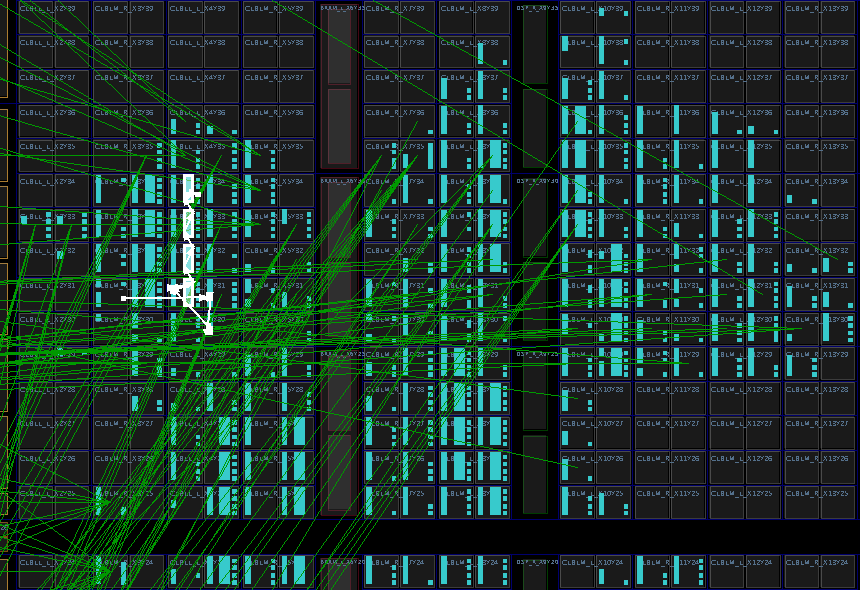
\includegraphics[width=0.9\textwidth]{./images/fig16_12_16_layout}
	\caption{\textit{Layout} de la implementación del algoritmo RC5-16/12/16.}
	\label{fig16_12_16_layout}
\end{figure}

\begin{figure}
	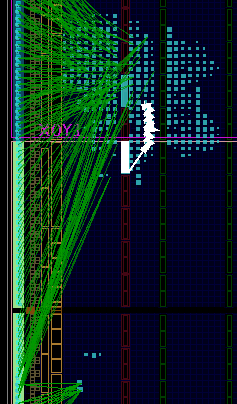
\includegraphics[width=0.9\textwidth]{./images/fig32_12_16_layout}
	\caption{\textit{Layout} de la implementación del algoritmo RC5-32/12/16.}
	\label{fig32_12_16_layout}
\end{figure}

\begin{figure}
	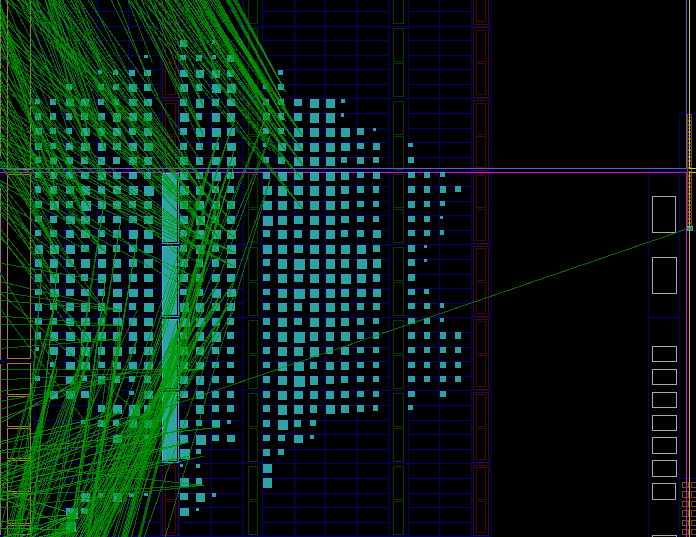
\includegraphics[width=0.9\textwidth]{./images/fig64_12_16_layout}
	\caption{\textit{Layout} de la implementación del algoritmo RC5-64/12/16.}
	\label{fig64_12_16_layout}
\end{figure}
%%%%%%%%%%%%%%%%%%%%%%%%%%%%%%%%%%
\begin{figure}[H]
	\centering
	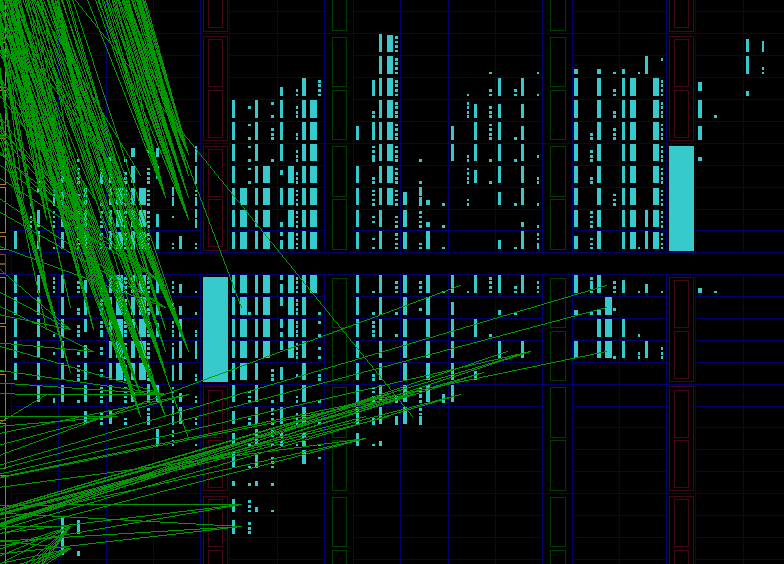
\includegraphics[width=0.85\textwidth]{./images/fig32_16_7_layout}
	\caption{\textit{Layout} de la implementación del algoritmo RC5-32/16/7.}
	\label{fig32_16_7_layout}
\end{figure}

\begin{figure}
	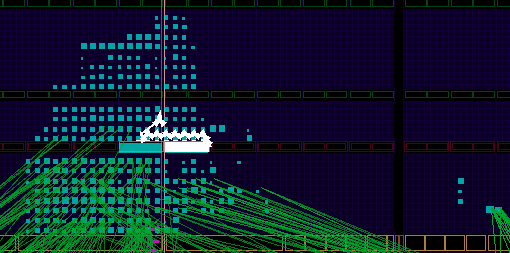
\includegraphics[width=1\textwidth]{./images/fig32_16_12_layout}
	\caption{\textit{Layout} de la implementación del algoritmo RC5-32/16/12.}
	\label{fig32_16_12_layout}
\end{figure}


\begin{figure}
	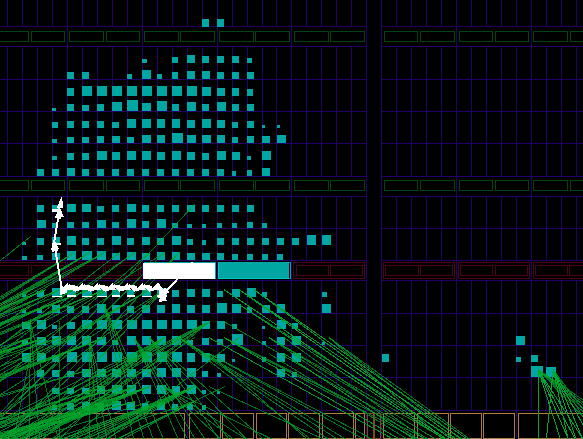
\includegraphics[width=0.9\textwidth]{./images/fig32_16_16_layout}
	\caption{\textit{Layout} de la implementación del algoritmo RC5-32/16/16.}
	\label{fig32_16_16_layout}
\end{figure}

Posterior a verificar el funcionamiento del algoritmo mediante se procedió a sintetizar e implementar el algoritmo (con las variaciones descritas en las Tablas \ref{tabSimRC51} y \ref{tabSimRC52}) haciendo uso del \textit{Vivado Design Suite}. Con esto se obtuvo la variación de recursos del FPGA mostrada en las Tablas \ref{tabVariacionRC5llave} y \ref{tabVariacionRC5palabra} mediante el mismo procedimiento descrito en la Sección \ref{resultadosAnalisisTEA}. En el caso de las variaciones de palabra se realizó de esta manera porque el autor del algoritmo indica que la implementación nominal del algoritmo es la RC5-32/12/16  y por tanto se quería observar la variación en el consumo de recursos alrededor del tamaño de palabra nominal, ajustandose a valores típicos de tamaños de palabra (potencias de 2). En el caso del tamaño de llave la variación se llevó a cabo de esta manera para poder realizar el análisis comparativo más adelante.

\begin{table}[htbp]
  \centering
    \begin{tabular}{rrrrrrrr}
    \toprule
    \begin{tabular}[c]{@{}l@{}}Tamaño\\llave\\(bytes)\end{tabular} & \begin{tabular}[c]{@{}l@{}}LUT as\\Logic\end{tabular} & RAM   & \begin{tabular}[c]{@{}l@{}}LUT as\\Memory\end{tabular} & Slice L & Slice M & \begin{tabular}[c]{@{}l@{}}Slice\\Regs\end{tabular} & \begin{tabular}[c]{@{}l@{}}Frec.\\máx.\\(MHz)\end{tabular} \\
    \midrule
    7    & 993   & 2     & 8     & 180   & 135   & 685   & 227,27 \\
    12    & 993   & 2     & 8     & 194   & 127   & 688   & 217,39 \\
    16    & 991   & 2     & 8     & 187   & 129   & 688   & 212,77 \\
    \bottomrule
    \end{tabular}%
  \caption{Variación del tamaño de la llave y recursos del FPGA para el algoritmo RC5-32/16/B}
  \label{tabVariacionRC5llave}%
\end{table}%

\begin{table}[htbp]
  \centering
    \begin{tabular}{rrrrrrrr}
    \toprule
    \begin{tabular}[c]{@{}l@{}}Tamaño\\palabra\\(bits)\end{tabular} & \begin{tabular}[c]{@{}l@{}}LUT\\as Logic\end{tabular} & RAM   & \begin{tabular}[c]{@{}l@{}}LUT as\\Memory\end{tabular} & Slice L & Slice M & \begin{tabular}[c]{@{}l@{}}Slice\\Regs\end{tabular} & \begin{tabular}[c]{@{}l@{}}Frec.\\máx.\\(MHz)\end{tabular} \\
   \midrule
    16    & 578   & 0     & 40    & 112   & 82    & 446   & 377,36 \\
    32    & 972   & 2     & 8     & 188   & 139   & 687   & 212,77 \\
    64    & 1911  & 4     & 8     & 314   & 236   & 1273  & 192,31 \\
    \bottomrule
    \end{tabular}%
  \caption{Variación del tamaño de la palabra y recursos del FPGA para el algoritmo RC5-W/12/16}
  \label{tabVariacionRC5palabra}%
\end{table}%

\subsection{Resultados y análisis de la variación del tamaño de la llave}

De la Tabla \ref{tabVariacionRC5llave} se generó la gráfica mostrada en la Figura \ref{figllaveRC5}. La gráfica muestra la viaración del consumo de recursos del FPGA y la frecuencia máxima de reloj conforme varia el tamaño de llave, el comportamiento mostrado fue casi constante demostrando que la variación del tamaño de la llave de un tamaño mayor al doble no afecta el consumo de recursos del FPGA. Esto es muy valioso debido a que al aumentar el tamaño de llave se aumenta la seguridad del algoritmo pero no afecta el consumo de recursos del FPGA. En el aspecto que si afecta esta variación es en la cantidad de tiempo de procesamiento, ya que se debe leer y escribir más veces a la memoria que resguarda la llave. Así se podría concluir del análisis que el tamaño de llave ideal depende de cuanta seguridad se quiere y que tan rápido se necesita llevar a cabo el proceso de cifrado/descifrado de los datos.

\begin{figure}[H]
	\centering
	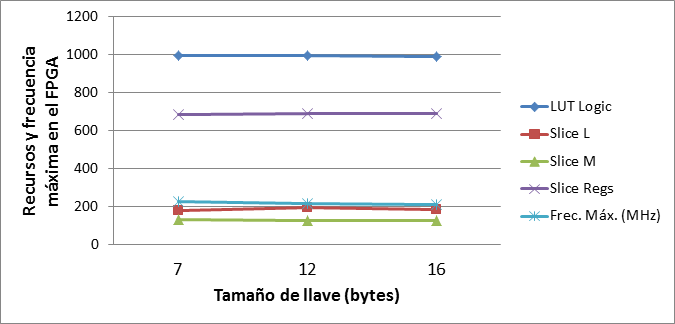
\includegraphics[width=0.8\textwidth]{./images/figLlaveRC5}
	\caption{Gráfica de consumo de recursos y frecuencia máxima del FPGA contra la variación del tamaño de llave en bytes al implementar el algoritmo RC5.}
	\label{figllaveRC5}
\end{figure}


\subsection{Resultados y análisis de la variación del tamaño de la palabra}
De la Tabla \ref{tabVariacionRC5palabra} se extrajeron las gráficas de la Figuras \ref{figSlicesRC5}, \ref{figSliceRegsLutsRC5}, \ref{figRamRC5} y \ref{figFrecuenciasRC5}. 

La Figura \ref{figSlicesRC5} muestra la variación de la cantidad de \textit{Slices L} y \textit{Slices M} consumidos conforme se varía el tamaño de palabra. Además la Figura \ref{figSliceRegsLutsRC5} muestra la variación de la cantidad de \textit{Slice Registers} y LUTs variando el tamaño de palabra. Como se puede observar de ambas figuras los datos muestran un comportamiento exponencial y similar, esto se debe a que, como se mencionó en el análisis del algoritmo TEA, los \textit{Slices} se componen de registros y LUTs.


\begin{figure}[H]
	\centering
	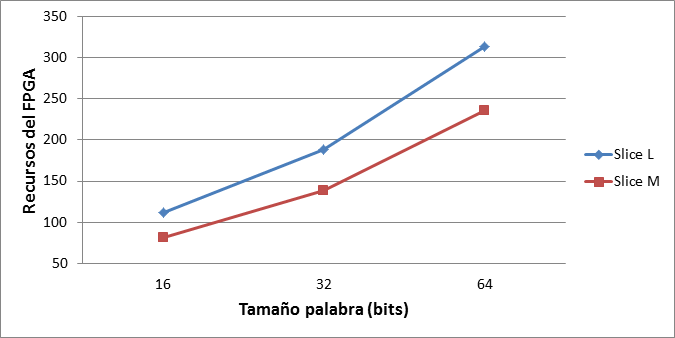
\includegraphics[width=0.8\textwidth]{./images/figSlicesRC5}
	\caption{Gráfica de consumo de \textit{Slices L} y \textit{Slices M} del FPGA contra la variación del tamaño de la palabra al implementar el algoritmo RC5.}
	\label{figSlicesRC5}
\end{figure}

\begin{figure}[H]
	\centering
	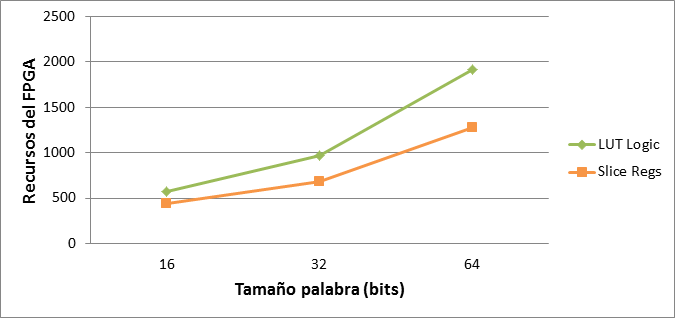
\includegraphics[width=0.8\textwidth]{./images/figSliceRegsLutsRC5}
	\caption{Gráfica de consumo de \textit{Slice Registers} y LUTs del FPGA contra la variación del tamaño de la palabra al implementar el algoritmo RC5.}
	\label{figSliceRegsLutsRC5}
\end{figure}

La Figura \ref{figRamRC5} muestra el consumo de \textit{LUT as memory} y bloques de memoria RAM al variar el tamaño de palabra. Como se puede observar, la implementación del algoritmo con tamaño de palabra de 16 bits no hace uso de ningún RAM y más bien utiliza LUTs como memoria. Posteriormente las otras dos implementaciones hacen uso de RAMs causando el desuso de gran parte de los LUTs utilizados como memoria, disminuyendo esta métrica de manera drástica y manteniéndola constante. Finalmente de la gráfica se puede observar el comportamiento lineal del consumo de bloques de memoria RAM ajustándose a lo esperado de que al duplicar el tamaño de palabra se duplique el uso de bloques de memoria RAM.
\begin{figure}[H]
	\centering
	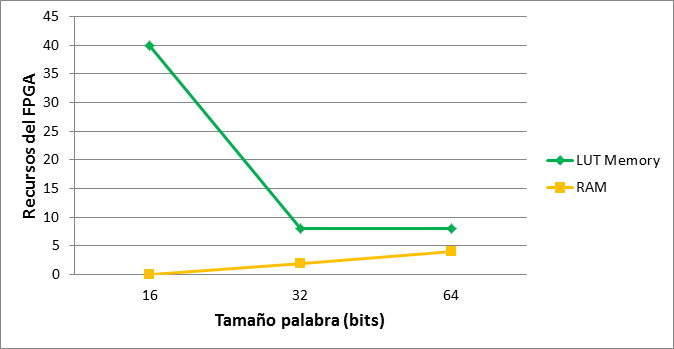
\includegraphics[width=0.8\textwidth]{./images/figRamRC5}
	\caption{Gráfica de consumo de \textit{LUT as memory} y bloques de memoria RAM del FPGA contra la variación del tamaño de la palabra al implementar el algoritmo RC5.}
	\label{figRamRC5}
\end{figure}

La Figura \ref{figFrecuenciasRC5} muestra la variación de la frecuencia máxima de reloj al variar el tamaño de palabra. Como se puede observar para la implementación de tamaño de palabra de 16 bits la frecuencia es mucho más alta que para las otras dos implementaciones. Esto se debe al cambio de utilizar LUTs como memoria a bloques de memoria RAM, los cuales son mucho más lentos. Además note como al pasar de 32 bits de tamaño de palabra a 64 bits, la variación de frecuencia máxima es pequeña, debido a que al no mapear la memoria a LUTs sino a bloques de memoria RAM no se tiene una memoria distribuida sino centralizada produciendo que la frecuencia sea mucho más estable.
\begin{figure}[H]
	\centering
	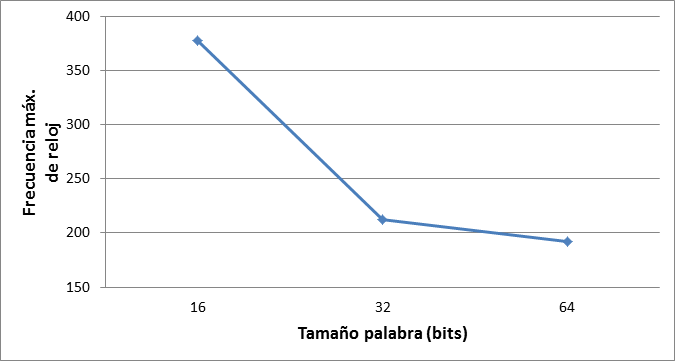
\includegraphics[width=0.8\textwidth]{./images/figFrecuenciasRC5}
	\caption{Gráfica de frecuencia máxima del FPGA contra la variación del tamaño de la palabra al implementar el algoritmo RC5.}
	\label{figFrecuenciasRC5}
\end{figure}

Finalmente y al igual que con el algoritmo TEA se normalizaron los datos para tener una visión global para analizar. Los datos normalizados se muestran en la Tabla \ref{tabNormalizadoRC5} y se reflejan en la Figura \ref{figNormalizadoRC5}. Se exceptúo del análisis normalizado las métricas \textit{LUT as memory} y RAM debido a que RAM no era un parámetro normalizable (para el tamaño de palabra de 16 bits es cero) y que \textit{LUT as memory} varió de forma inconsistente por el uso de bloques de memoria RAM, agregando poco valor al análisis. De la gráfica se observa VOY A AGUANTARLA A HABLAR CON EL PROFE PORQUE LA GRAFICA SE COMPORTA IGUAL A LA DEL TEA.

\begin{table}[htbp]
  \centering
    \begin{tabular}{rrrrrr}
    \toprule
    \begin{tabular}[c]{@{}l@{}}Tamaño\\palabra\\(bits)\end{tabular} & \begin{tabular}[c]{@{}l@{}}LUT\\as Logic\end{tabular} &   Slice L & Slice M & \begin{tabular}[c]{@{}l@{}}Slice\\Regs\end{tabular} & \begin{tabular}[c]{@{}l@{}}Frec.\\máx.\\(MHz)\end{tabular} \\
   \midrule
    16    & 1     & 1     & 1     & 1     & 1,96 \\
    32    & 1,68  & 1,68  & 1,70  & 1,54  & 1,11 \\
    64    & 3,31  & 2,80  & 2,88  & 2,85  & 1 \\
    \bottomrule
    \end{tabular}%
  \caption{Variación del tamaño de la palabra y recursos del FPGA normalizados para el algoritmo RC5-W/12/16.}
  \label{tabNormalizadoRC5}%
\end{table}%

\begin{figure}[H]
	\centering
	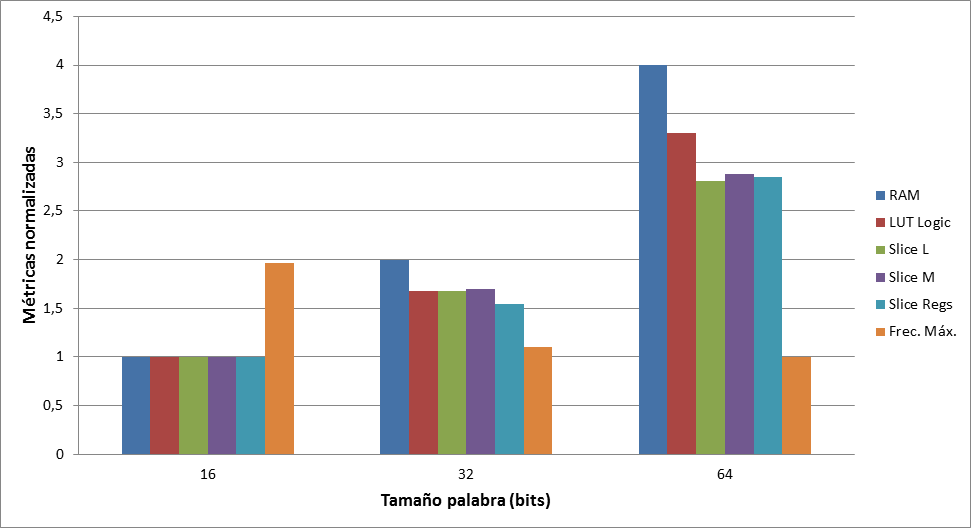
\includegraphics[width=1\textwidth]{./images/figNormalizadoRC5}
	\caption{Gráfica de consumo de recursos y frecuencia máxima (normalizados respecto al valor mínimo) del FPGA contra la variación del tamaño de palabra al implementar el algoritmo RC5.}
	\label{figNormalizadoRC5}
\end{figure}


\clearpage
\section{Análisis comparativo}
Para realizar el análisis comparativo es necesario tener un punto de referencia para la escogencia de los parámetros de cada algoritmo con el fin de lograr un análisis justo. Esto se logró tomando como referencia lo descrito en los artículos que describen cada algoritmo. En ambos artículos se hace una referencia a cual implementación del algoritmo es ``equivalente'' a utilizar el algoritmo DES. Citando ambos artículos:
\cite{rivest}
    \emph{``As an example, consider the problem of replacing DES with an "equivalent" RC5 algorithm. One might reasonable choose RC5-32/16/7 as such a replacement.''}

\cite{tea}
   \emph{``This type of algorithm can replace DES in software, and is short enough to write into almost any program on any computer.''}
 
Por tanto el RC5-32/16/7 y el TEA con 32 rondas y tamaño de palabra de 32 bits fueron elegidos para realizar el análisis comparativo.
	
	%resultados
	%\chapter{Resultados}

\section{Pruebas para comprobar la funcionalidad y estabilidad}

Al finalizar el desarrollo de la aplicación, se probó acceder a ella desde computadoras en diferentes sistemas operativos. En todos los casos la aplicación operaba de forma correcta. Por lo que independientemente del OS del sistema, la herramienta es funcional, dando como resultado una aplicación web, multiplataforma. Lo cual era uno de los objetivos que se quería alcanzar inicialmente.\\

Además se analizó la exactitud de los datos obtenidos. A la hora de realizar los contornos con la herramienta desarrollado, siempre se obtuvo todos los pixeles que forman parte del mismo, distinto a Sensarea que se obtenían muy pocos puntos si se realizaba la funcionalidad de esta misma manera (dejando precionado el click izquierdo y desplazando el puntero al rededor del contorno).


\section{Pruebas realizadas por diversos usuarios}

Para probar que la aplicación diseñada en efecto es más sencilla de utilizar que las otras herramientas actuales y que con ella se generan datos de manera más eficiente, se procedió a realizar unas pruebas con tiempo a tres diferentes usuarios y se promedió el resultado. Las otras dos herramientas con las cuales se comparó fueron Sensara y VideoANT, debido a que son las únicas que no se requiere de conocimiento técnico para poder instalarlas o utilizarlas en línea. A cada uno se les solicitó realizar las siguientes tareas en orden:

\begin{enumerate}
\item Instalar o acceder a la aplicación
\item Abrir la aplicación, cargar uno de sus video y realizar la segmentación temporal de 5 escenas diferentes.
\item Seguir de la trayectoria de 5 elementos diferentes por al menos 20 cuadros.
\item Dibujar los contornos de 5 elementos diferentes por al menos 20 cuadros.
\item Realizar anotaciones semánticas de 5 tipos diferentes de escenas encontradas.
\end{enumerate}

El video que se utilizó fue una sección de la final de la Copa del Mundo Fifa 2010 entre España y Holanda. El peso del video es de 250 Mb, el formato es mp4 y codec es h264. Los resultados obtenidos se muestran en las tablas \ref{table:results} y \ref{table:results2}. La primera de ellas muestra lo que se duró haciendo la labor por primera vez y en la segunda tabla se muestra el valor promedio de tiempos en las 5 tareas de cada tipo.


\begin{table}[h]\centering
	
	\ra{2}
	\caption{Promedio de tiempo estimado de la primera función realizada correctamente}
	\label{table:results}
	
	\begin{tabular}{@{}cC{3cm}C{3cm}C{3cm}C{3cm}c@{}}\toprule
		
		& Función & GT-Tool & Sensarea & VideoANT&\\ \midrule
		
		& Primer uso de la aplicación & 7 segundos* & 2 minutos & 5 segundos* & \\
		
		& Segmentación temporal  & 26 segundos & 87 segundos & 15 segundos & \\
		
		& Rastreo de objetos & 5 segundos & 5 segundos & no aplica & \\
		
		& Segmentación de contornos & 27 segundos  & 34 segundos & no aplica & \\
		
		& Segmentación semántica & 20 segundos  & no aplica & 15 segundos & \\ 
		
		\bottomrule
		
	\end{tabular}
	
\end{table}

*Ese el tiempo que les tomó acceder a la página web, de lo contrario es el tiempo de descarga e instalación.\\

Se puede apreciar de esta primera tabla (\ref{table:results}), que GT-Tool es muy similar a Sensarea cuando se quiere realizar el seguimiento de la trayectoria de los objetos. Y es un poco más lento que VideoANT a la hora de realizar la segmentación temporal y semántica, esto es debido a la forma en la que VideoANT solicita la información, es más directa pero no tan especializada. De nuevo, VideoANT da precisión de segundos y no de cuadros y además no tiene manera de realizar seguimiento de trayectorias ni segmentación de contornos.\\

A continuación el promedio de las 5 repeticiones luego de haber realizado la tarea por primera vez:


\begin{table}[h]\centering
	
	\ra{2}
	\caption{Promedio de tiempo que tomó realizar cada función repetidas veces (5 repeticiones)}
	\label{table:results2}
	
	\begin{tabular}{@{}cC{3cm}C{3cm}C{3cm}C{3cm}c@{}}\toprule
		
		& Función & GT-Tool & Sensarea & VideoANT&\\ \midrule
		
		& Segmentación temporal  & 19 segundos & 30 segundos & 13 segundos & \\
		
		& Rastreo de objetos & 3 segundos & 4 segundos & no aplica & \\
		
		& Segmentación de contornos & 14 segundos  & 29 segundos & no aplica & \\
		
		& Segmentación semántica & 15 segundos  & no aplica & 13 segundos & \\ 
		
		\bottomrule
		
	\end{tabular}
	
\end{table}

Al analizar los resultados de dicha tabla se concluye los siguiente:

\begin{enumerate}
	
\item A medida que utilizan cualquier herramienta, el tiempo que les toma realizar una labor disminuye, sin importar cual sea. La disminución más grande la tuvo Sensarea en la segmentación temporal, pero esto fue debido a que, aunque Sensarea no soporta nativamente algún tipo de segmentación temporal, se puede simular colocando puntos con etiquetas. Cuando los usuarios se dieron cuenta de esto, lo empezaron a hacer y así hacían un tipo de segmentación temporal.

\item VideoANT continua siendo un poco más rápida para lo temporal y semántico, pero no cuenta con los otros tipos. De igual manera la diferencia en tiempos no es muy significativa.

\item GT-Tool si logra disminuir el tiempo en el que se generan los datos para la trayectoria de objetos y segmentación de contornos, mientras que a la vez aumenta la precisión brindada por Sensarea.

\end{enumerate}
	
	%conclusiones
	%\chapter{Conclusiones y recomendaciones}
\section*{Conclusiones}

\begin{itemize}
\item Fue posible implementar 2 algoritmos criptográficos en un FPGA haciendo uso del lenguaje de descripción de hardware Verilog.

\item De los análisis individuales podemos concluir que:
\begin{itemize}
\item El consumo de \textit{slice L}, \textit{slice M}, \textit{slice registers} y \textit{LUTs as logic} crece exponencialmente conforme se varía el tamaño de palabra.
\item En el caso del algoritmo RC5 se puede concluir que la variación del tamaño de llave no afecta el consumo de recursos del FPGA y que la variación en la frecuencia máxima tiene un comportamiento exponencial inverso.
\item La variación del tamaño de llave en el algoritmo RC5 afecta de forma mínima el consumo de recursos del FPGA.
\item En el caso del algoritmo TEA la frecuencia máxima tiene un comportamiento lineal decreciente.
\item Idealmente el algoritmo TEA debe ser implementado para tamaños de palabra menores o iguales a 32 bits, realizando un análisis entre cuanta seguridad y velocidad se desea.
\end{itemize}


\item Del análisis comparativo se puede concluir que de ambos algoritmos, el que consume la menor cantidad de recursos y presenta la mayor frecuencia de reloj es el TEA con 32 bits de tamaño de palabra y 32 rondas. Esto usando como referencia los artículos que describen ambos algoritmos para elegir el punto comparativo del algoritmo DES.
\end{itemize}

\section*{Recomendaciones}

\begin{itemize}
\item Agregar a las métricas de análisis, el tiempo de procesamiento en ciclos de reloj de cada una de las implementaciones realizadas.
\item Mejora el diseño mediante el uso de \textit{pipeline}, esto mejorará el desempeño de los algoritmos y se podría estudiar como este cambio impacta en las métricas analizadas por este trabajo.
\item Se prodría profundizar más en el desarrollo y diseño con FPGAs para habilitar el uso de bloques de DSP del mismo y así mejorar el desempeño y consumo de los algoritmos. Esto para explotar las capacidades de un FPGA.
\item Realizar un estudio previo sobre criptografía y más que todo sobre criptoanálisis para tener un mejor criterio sobre como afectan las variaciones del tamaño de palabra, número de rondas y el tamaño de llave en la seguridad del algoritmo.
\end{itemize}

	
	%--------------------------------------------------------------------
	%bibliografía
	\bibliography{eieclases_ref}
	%\cleardoublepage
	
	%--------------------------------------------------------------------
	%apéndice
	%\appendix
	
	%\chapter{Apéndice}
Con la finalidad de cuidar el ambiente ahorrando papel, el código realizado se encuentra disponible en \url{https://github.com/aglt93/proyectoElectrico}.
	%\include{apendice1}
	%\include{apendice2}
	
	%final del documento
\end{document}
